\chapter{Security Evidence Package}

\section{Frontend Security Evidence}

\subsection{SE-1: S3 Block Public Access enabled}
\begin{figure}[H]
    \centering
    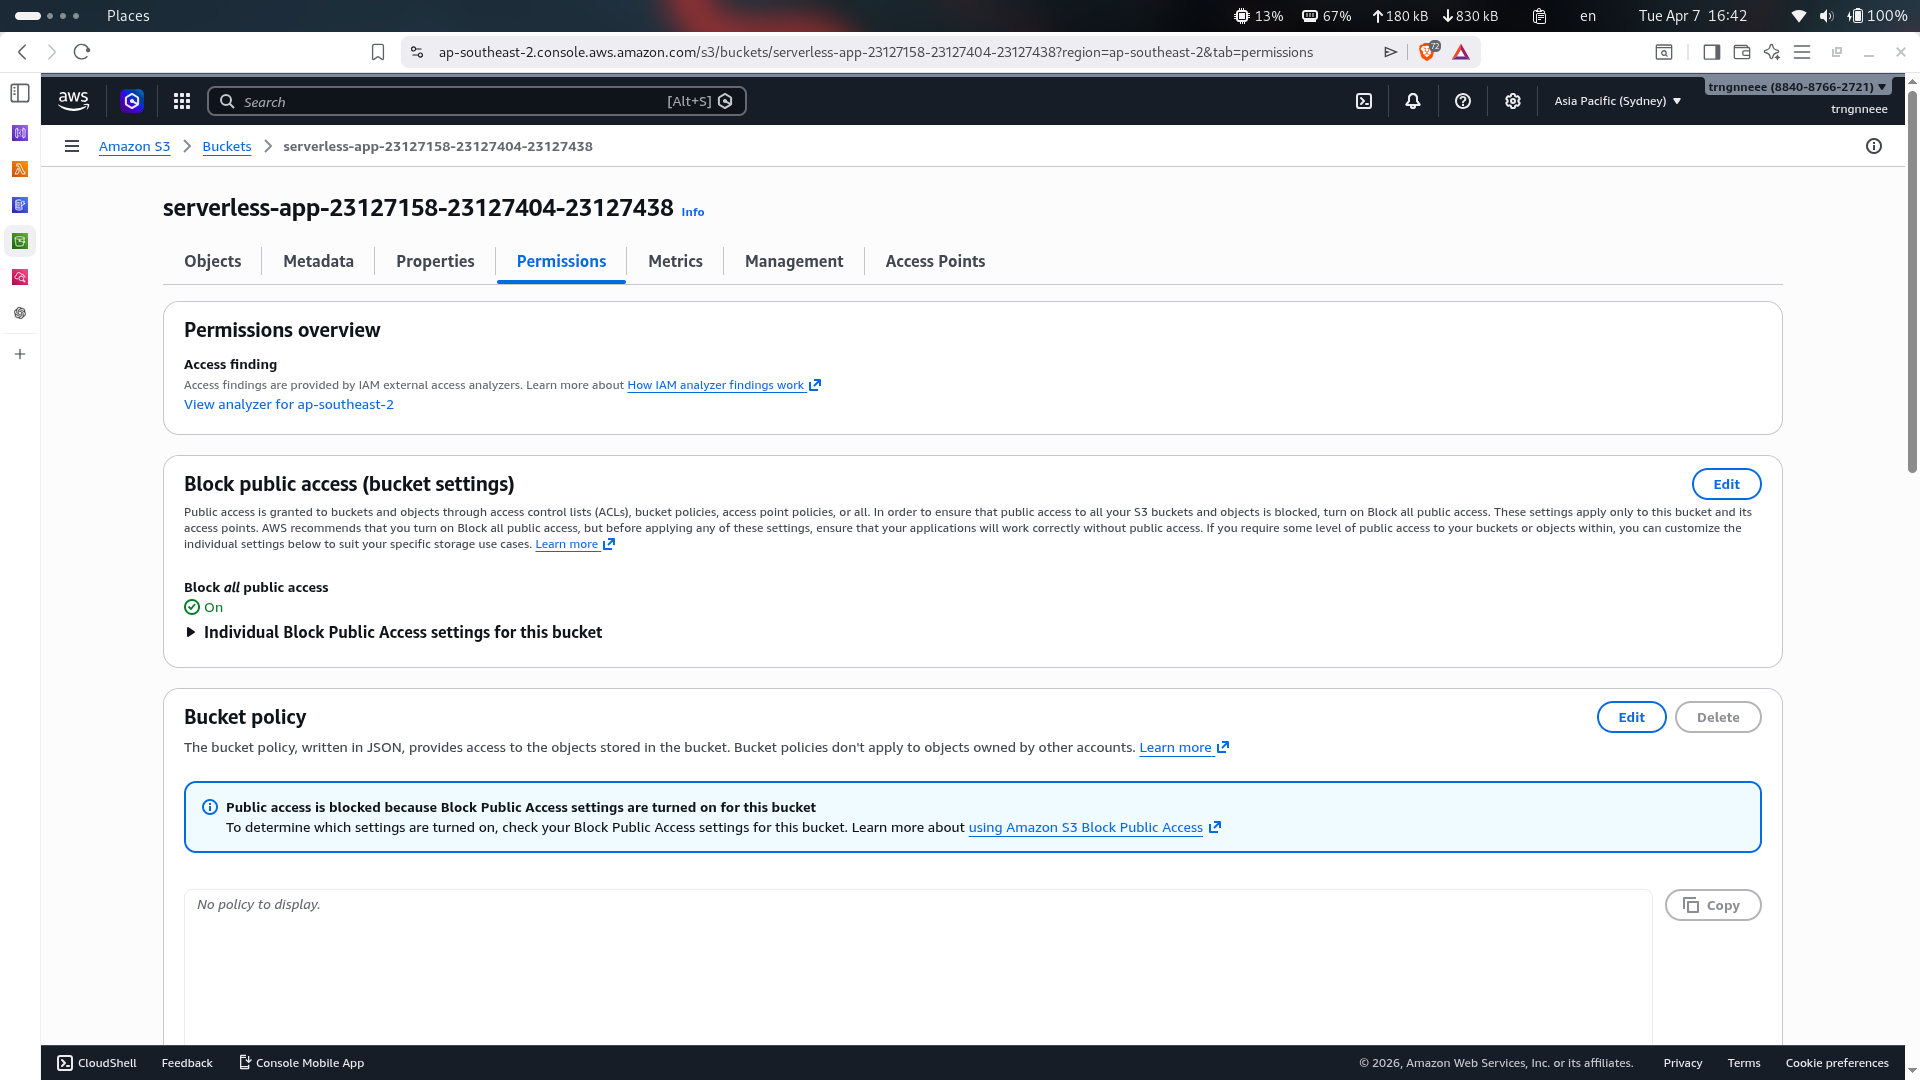
\includegraphics[width=0.8\textwidth]{images/SE1.png}
    \caption{SE-1}
\end{figure}

\subsection{SE-2: Direct S3 access rejected}
\begin{figure}[H]
    \centering
    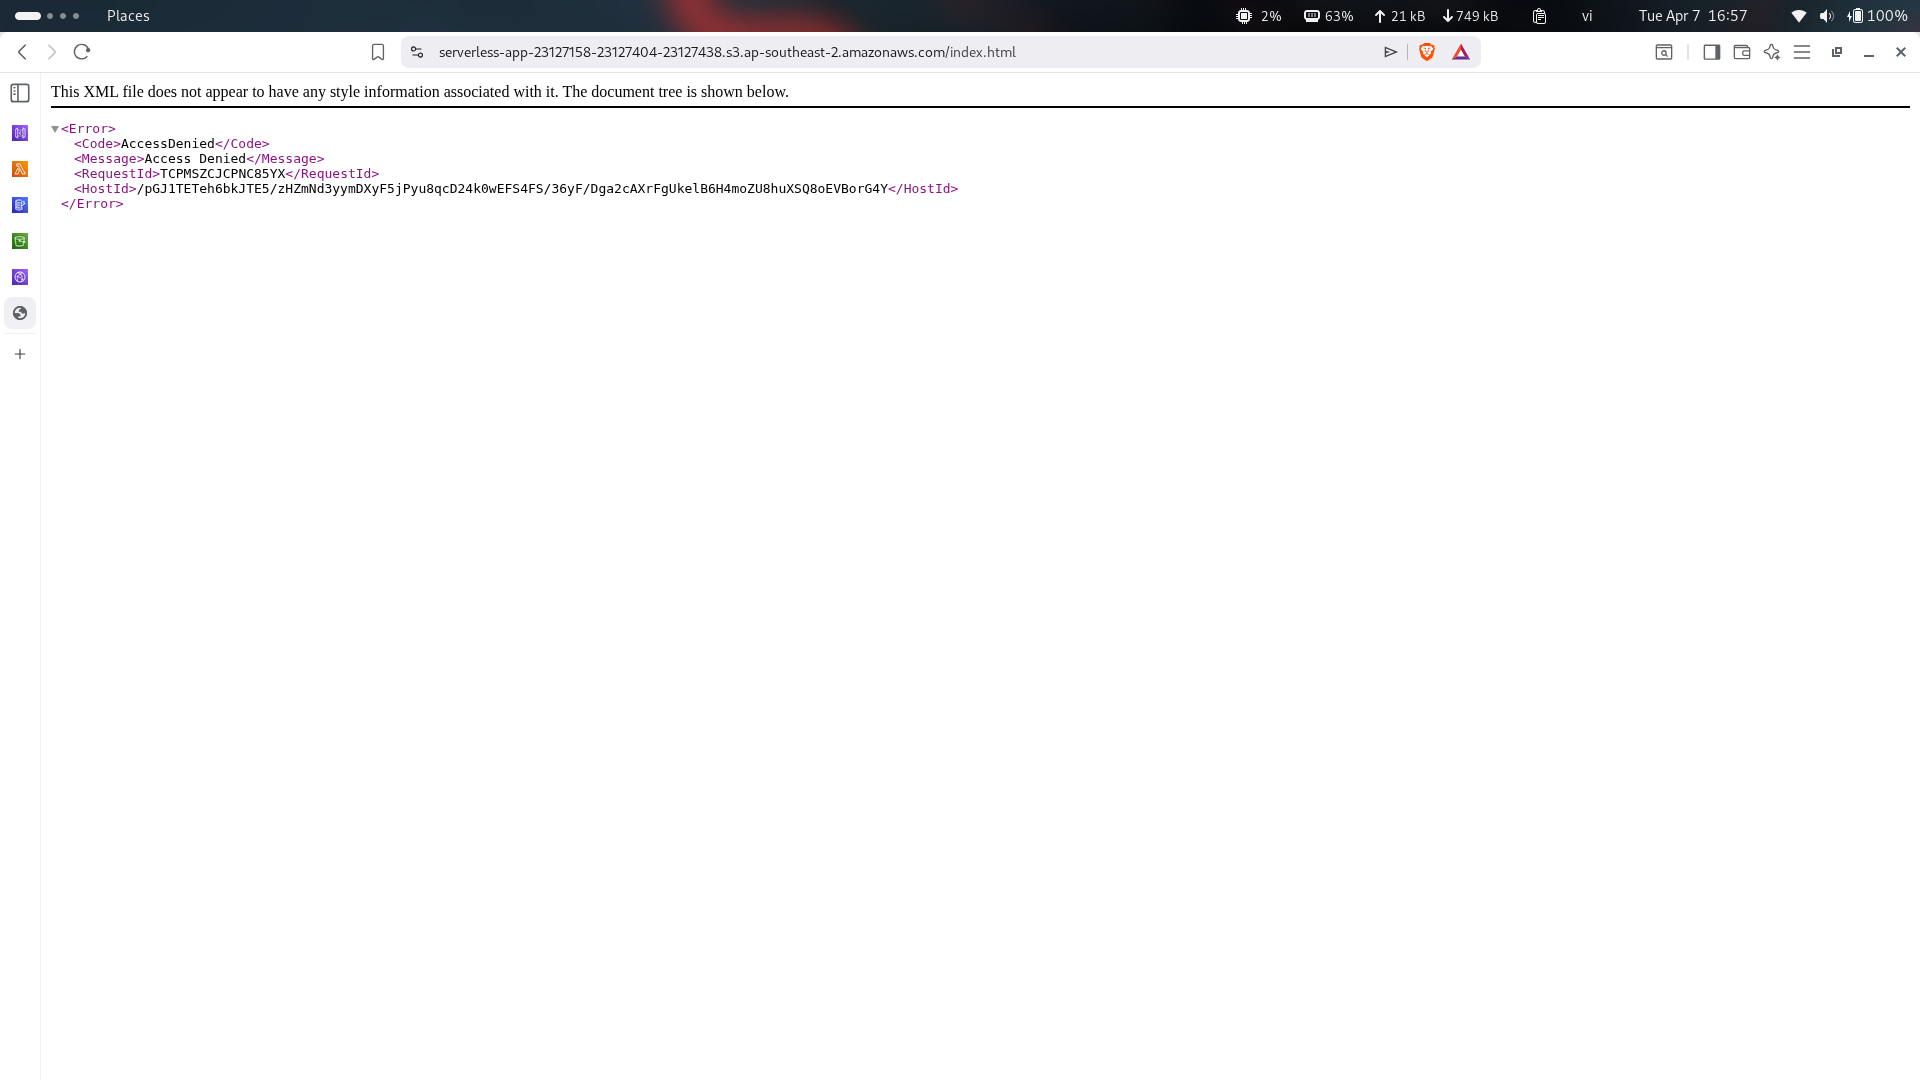
\includegraphics[width=0.8\textwidth]{images/SE2.png}
    \caption{SE-2}
\end{figure}

\subsection{SE-3: CloudFront access succeeds}
\begin{figure}[H]
    \centering
    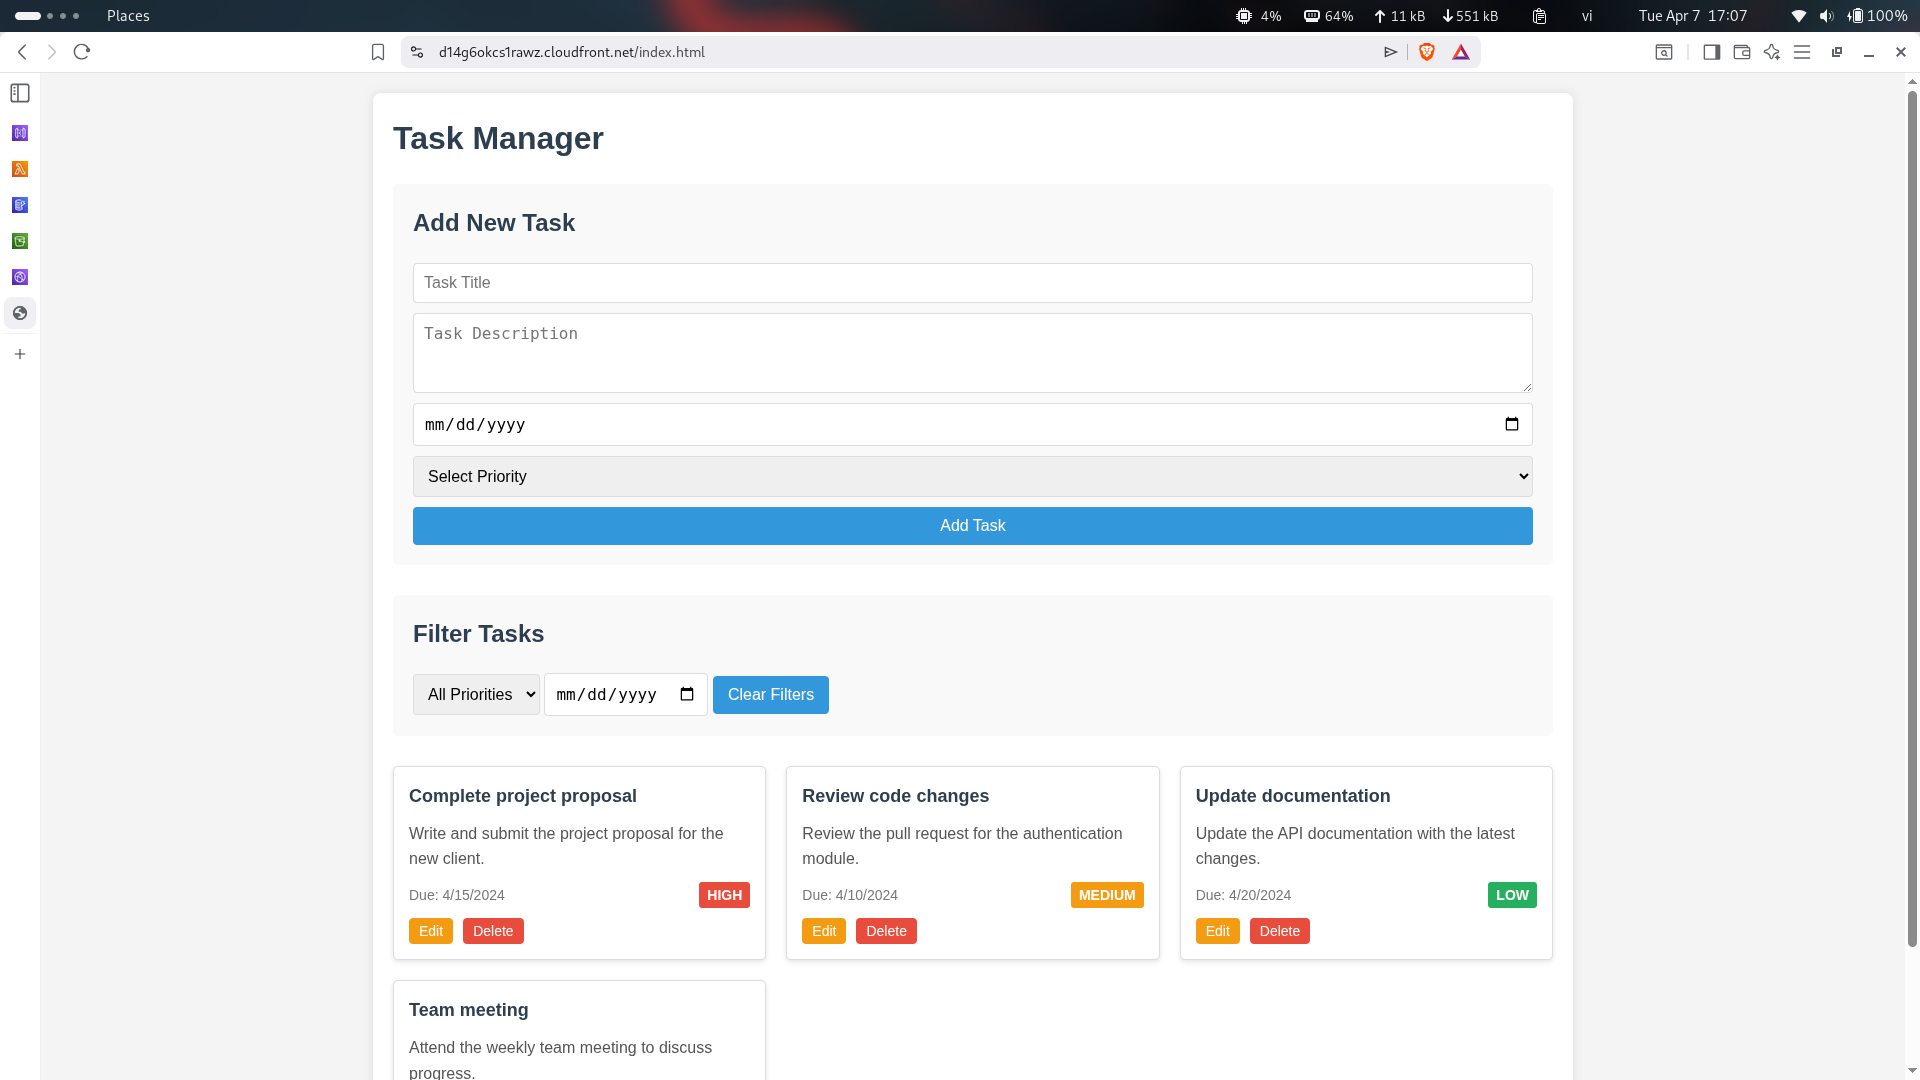
\includegraphics[width=0.8\textwidth]{images/SE3.png}
    \caption{SE-3}
\end{figure}

\subsection{SE-4: OAC attached to CloudFront}
\begin{figure}[H]
    \centering
    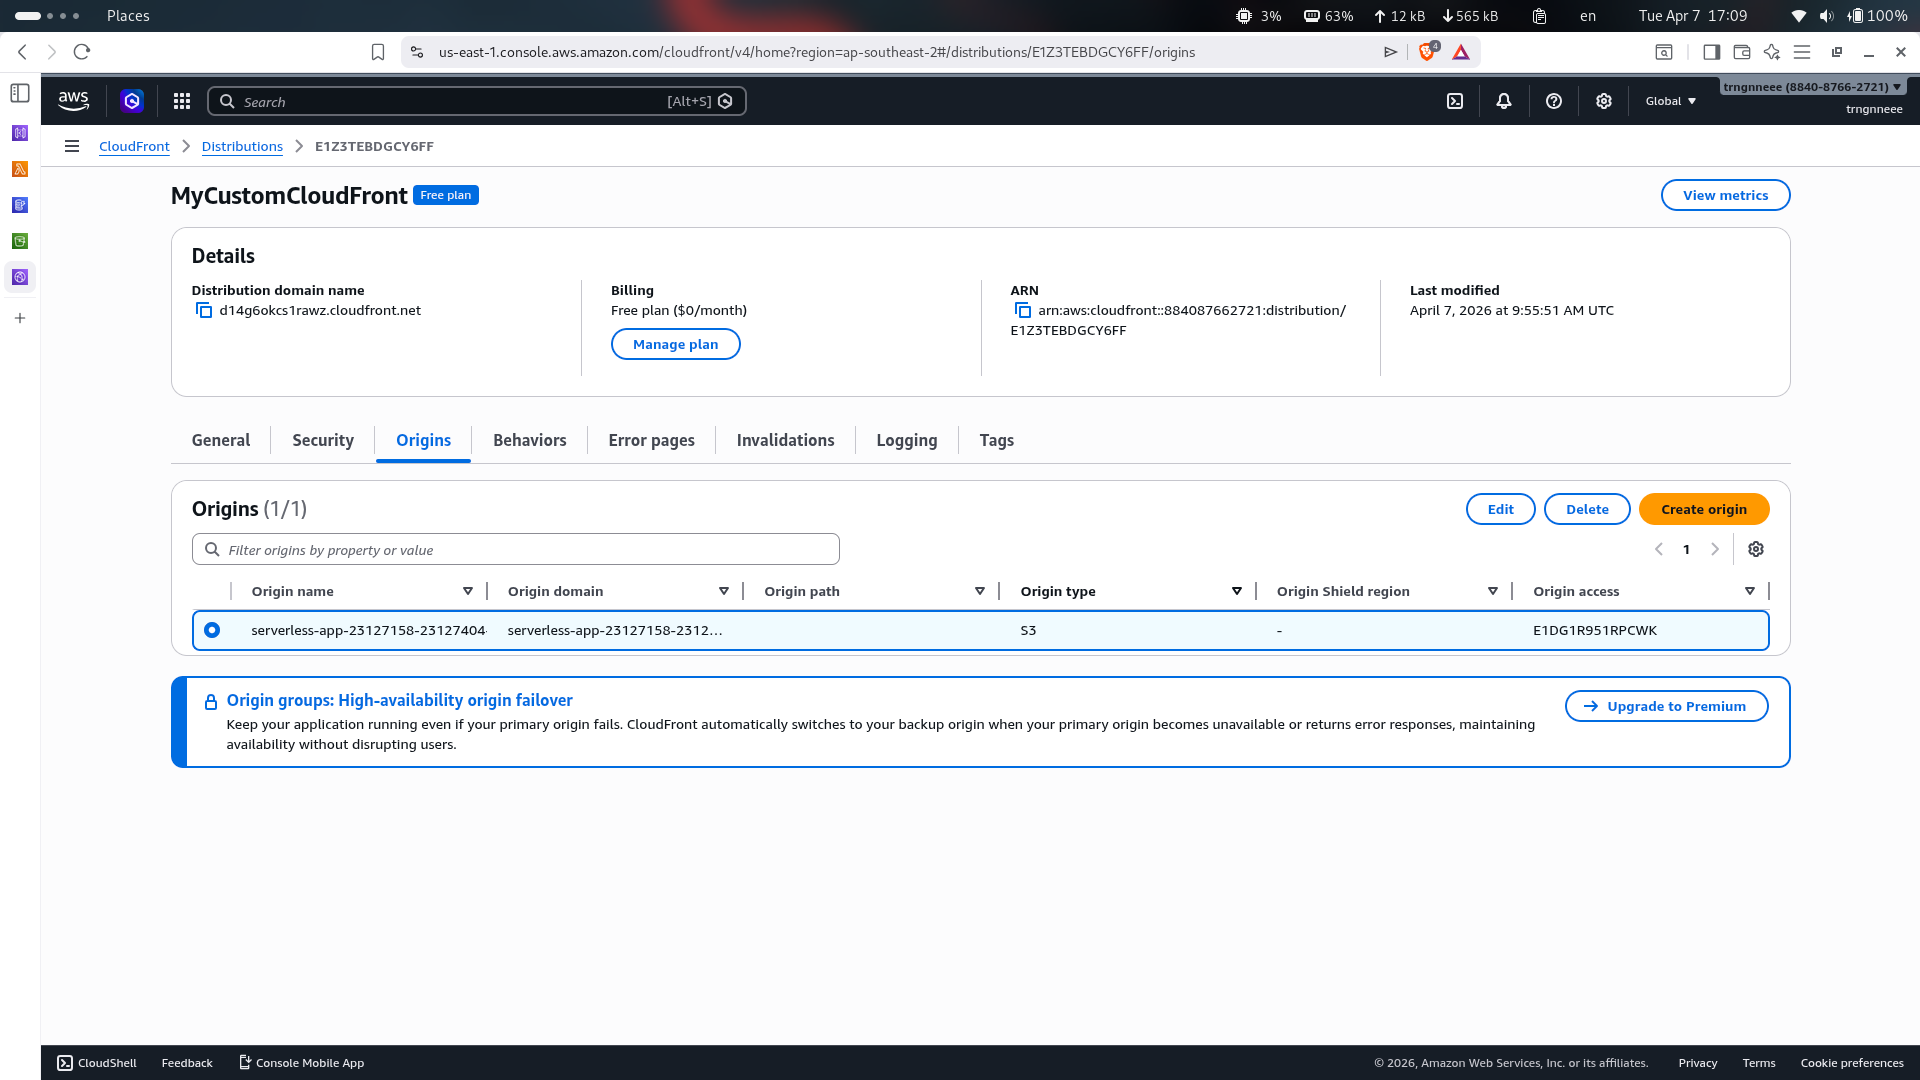
\includegraphics[width=0.8\textwidth]{images/SE4-1.png}
    \caption{Origins Access List}
\end{figure}

\begin{figure}[H]
    \centering
    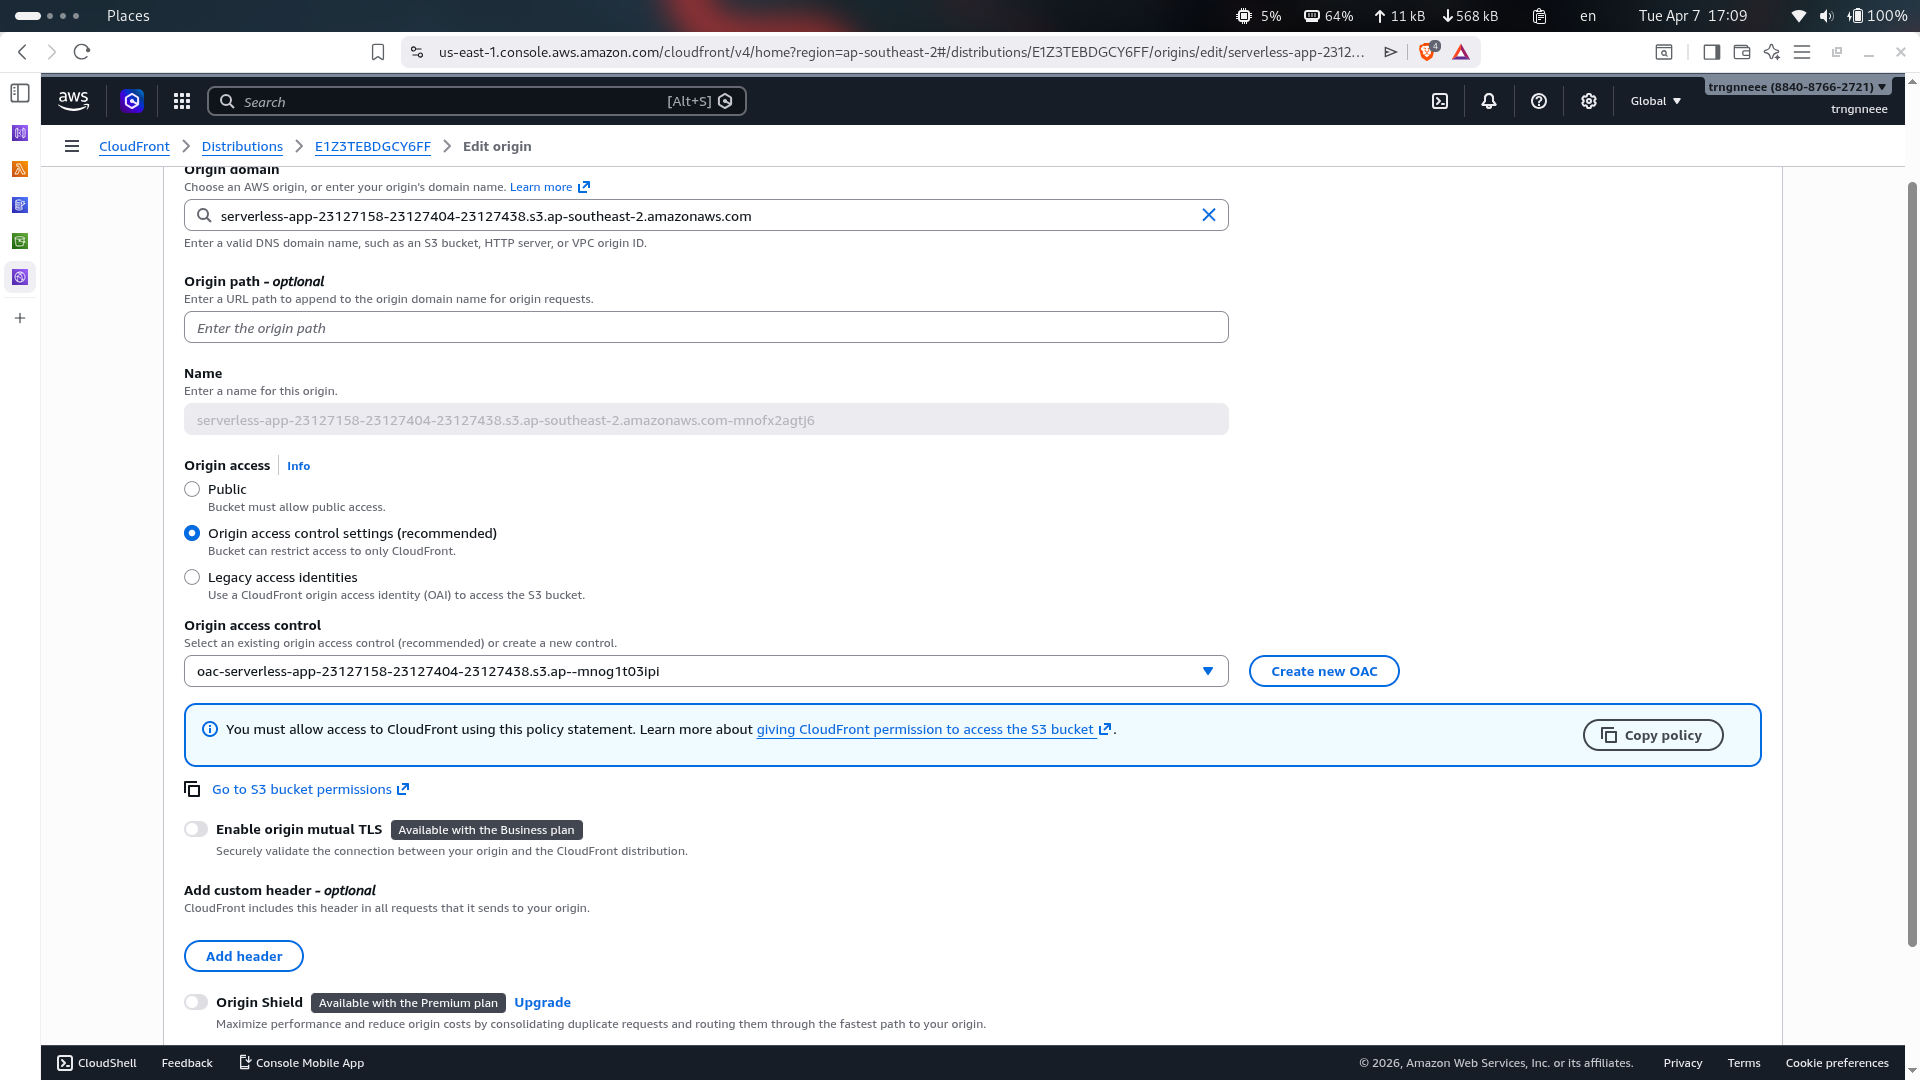
\includegraphics[width=0.8\textwidth]{images/SE4-2.png}
    \caption{Origins Access Setting}
\end{figure}

\section{Network Evidence}

\subsection{NE-1: VPC Endpoint created for DynamoDB}
\begin{figure}[H]
    \centering
    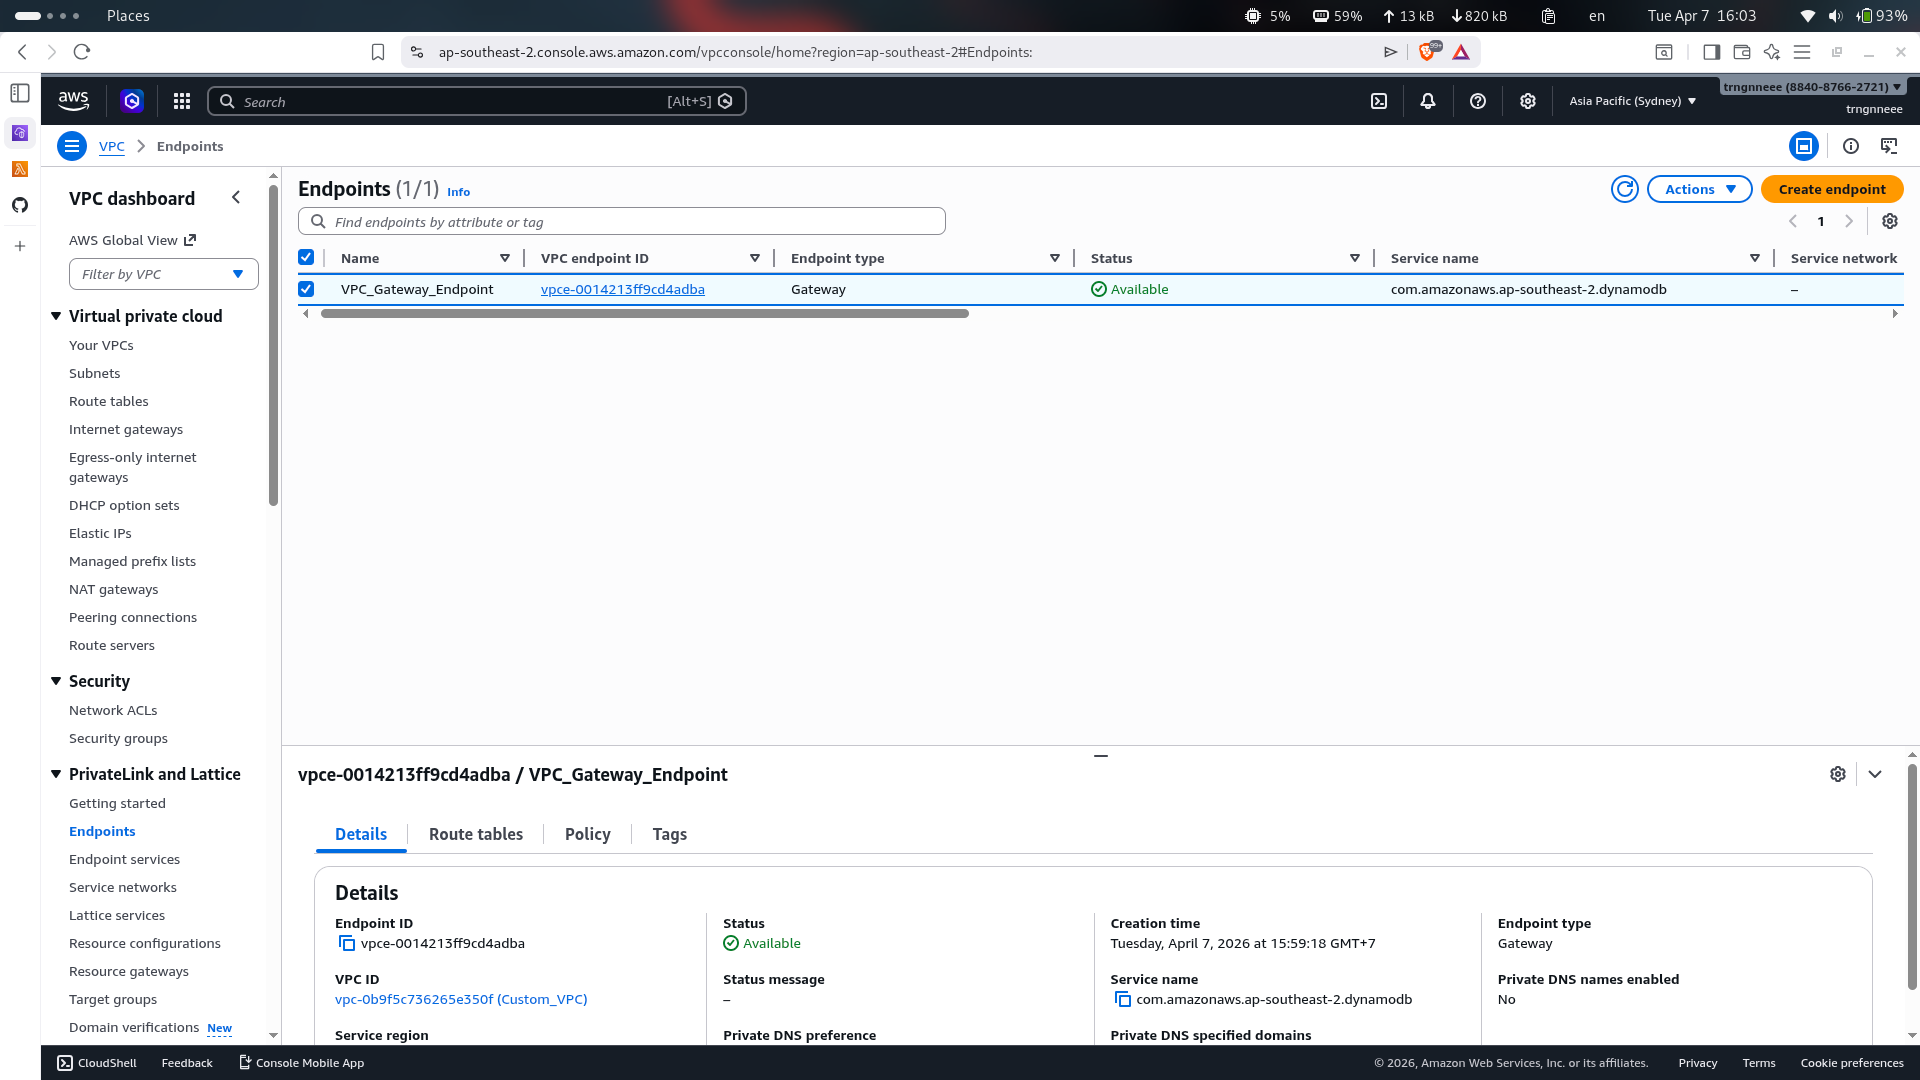
\includegraphics[width=0.8\textwidth]{images/NE1.png}
    \caption{NE-1}
\end{figure}

\subsection{NE-2: Lambda has VpcConfig}
\begin{figure}[H]
    \centering
    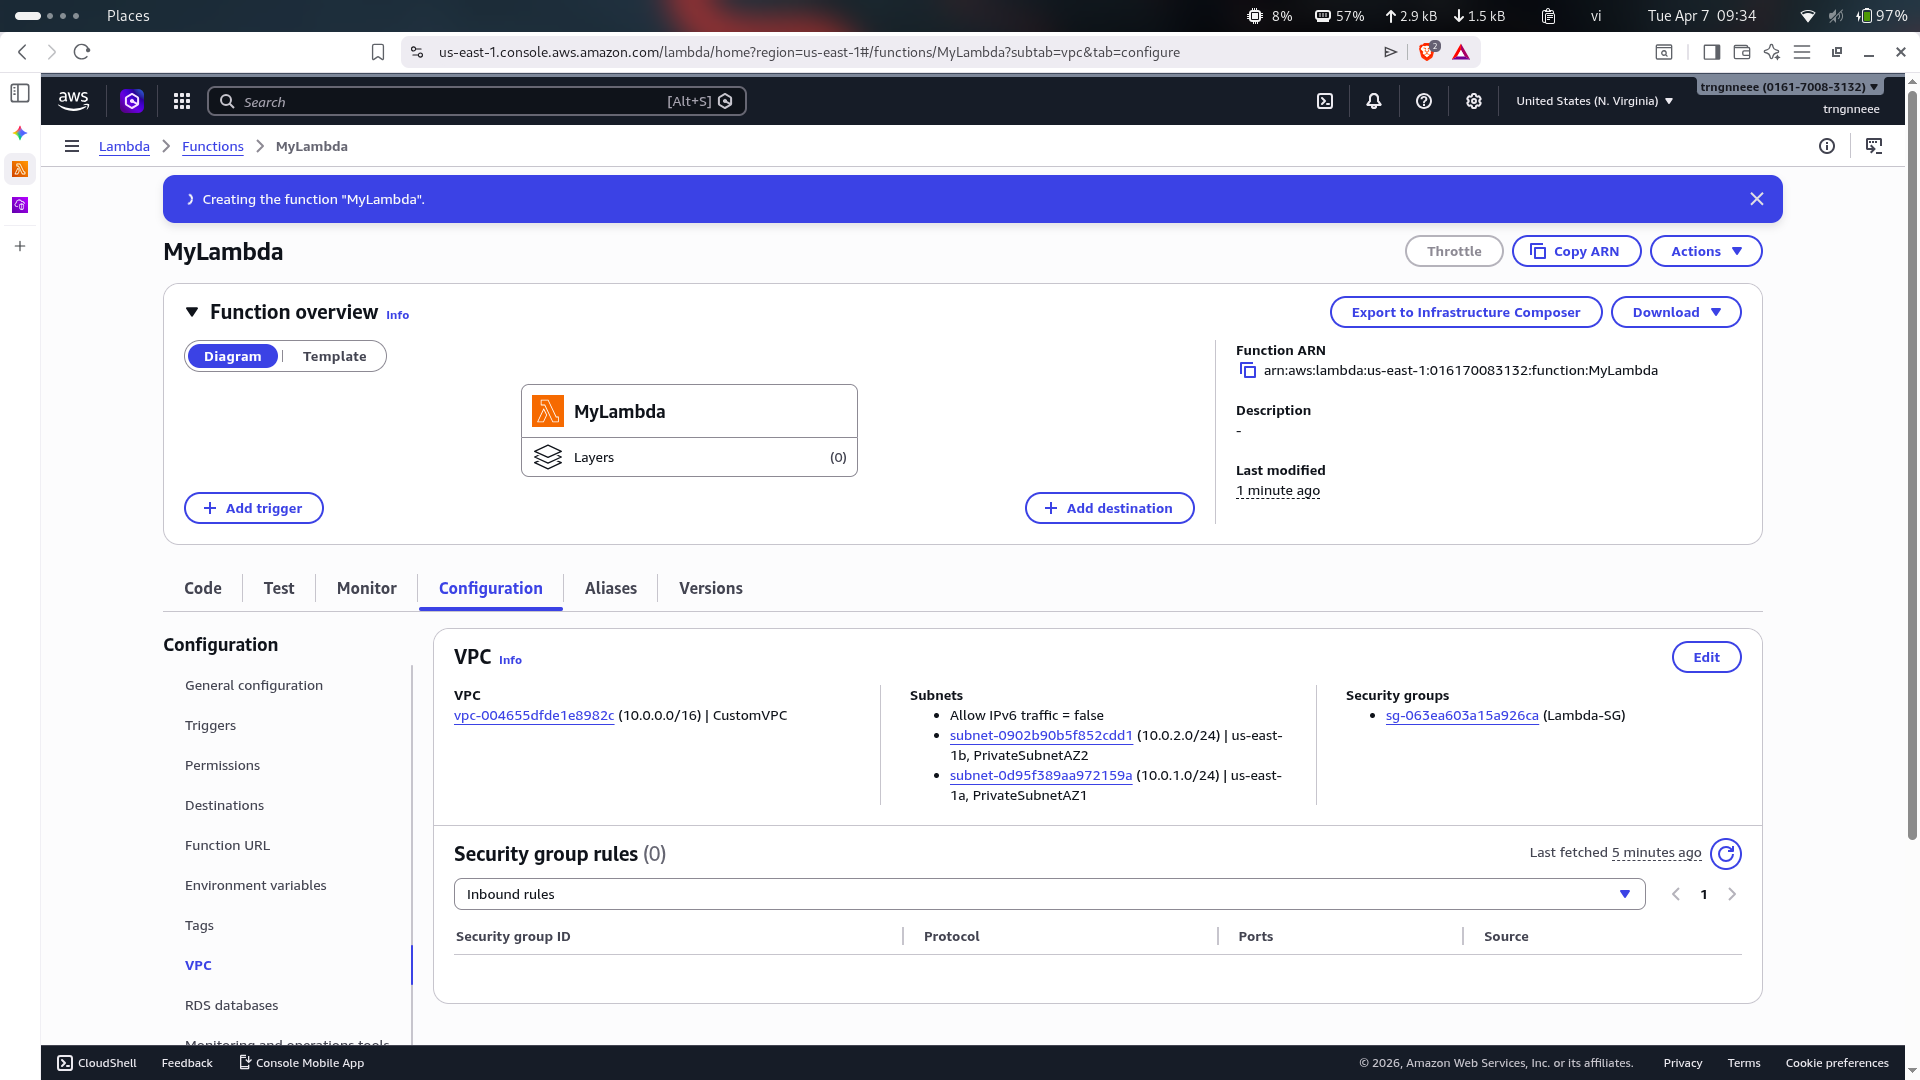
\includegraphics[width=0.8\textwidth]{images/NE2.png}
    \caption{NE-2}
\end{figure}

\subsection{NE-3: Route table has Endpoint route}
\begin{figure}[H]
    \centering
    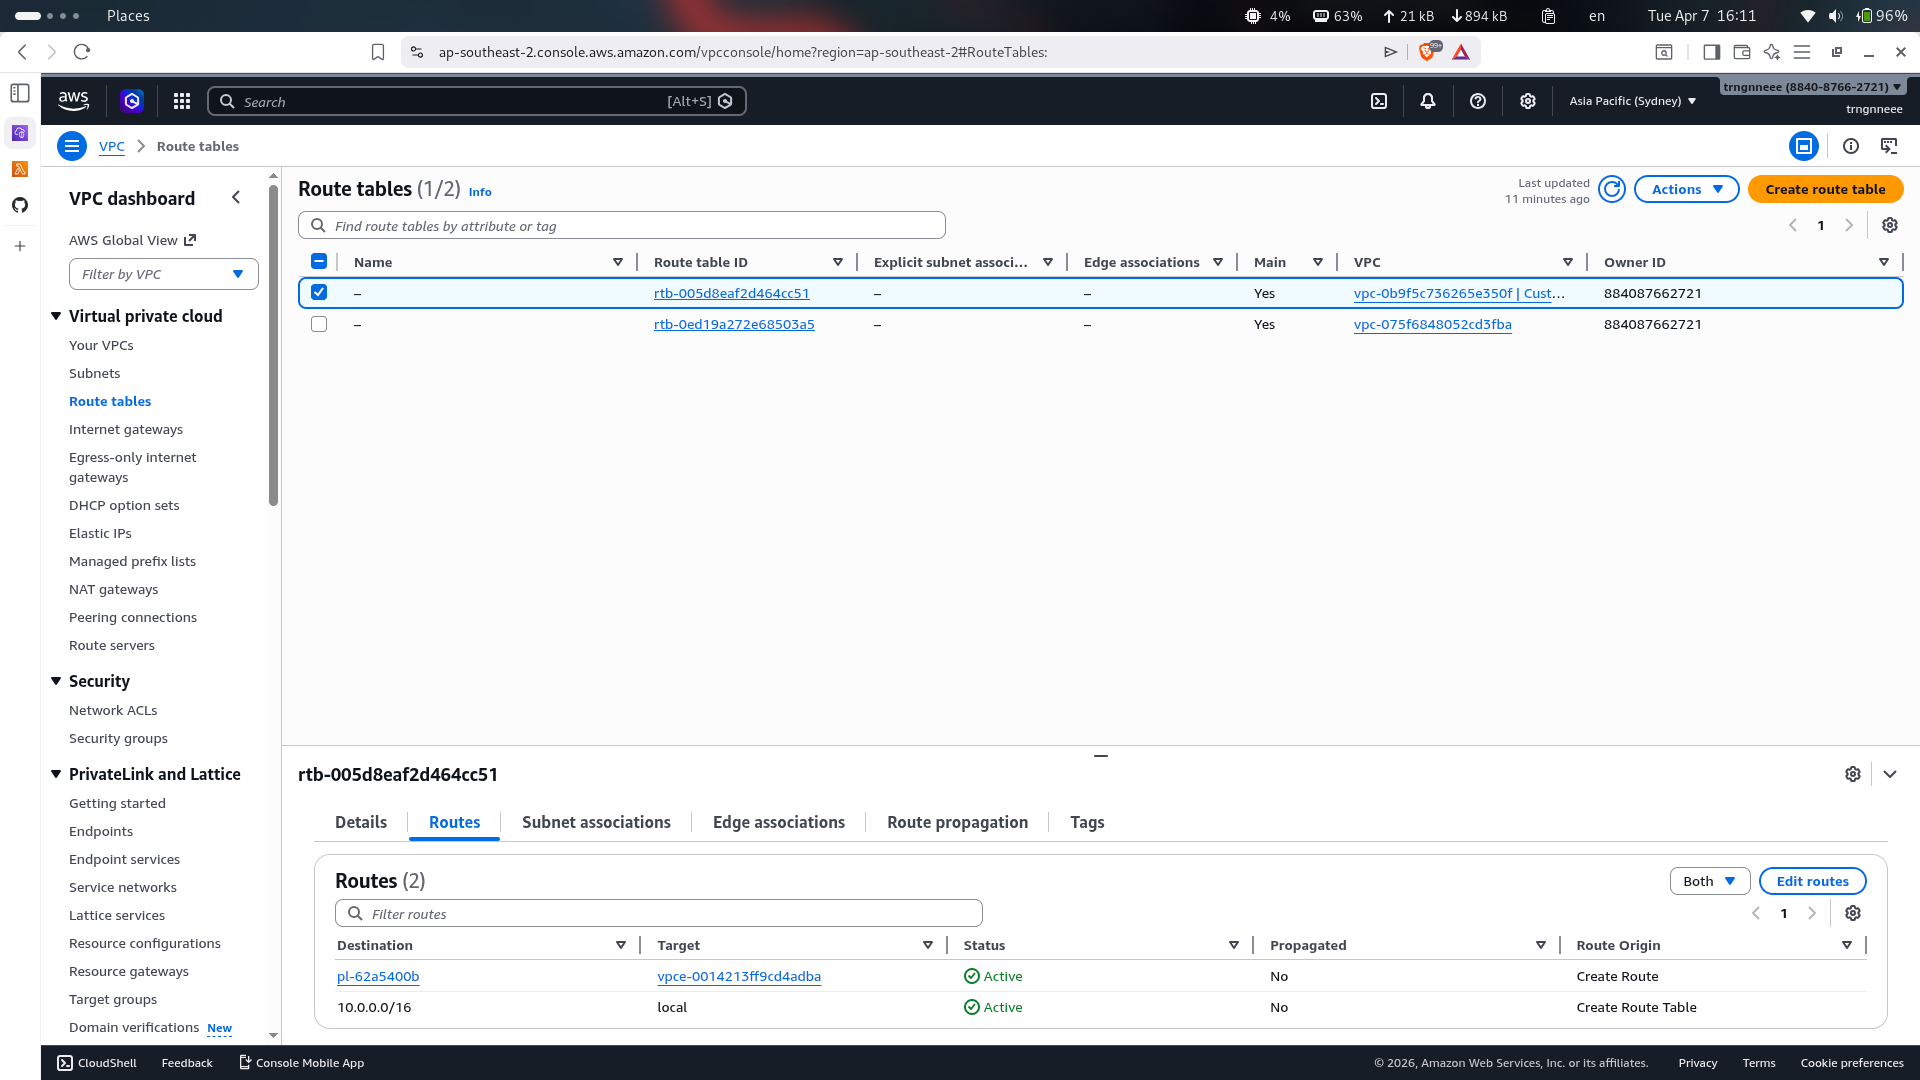
\includegraphics[width=0.8\textwidth]{images/NE3.png}
    \caption{NE-3}
\end{figure}

\subsection{NE-4: No NAT Gateway exists}
\begin{figure}[H]
    \centering
    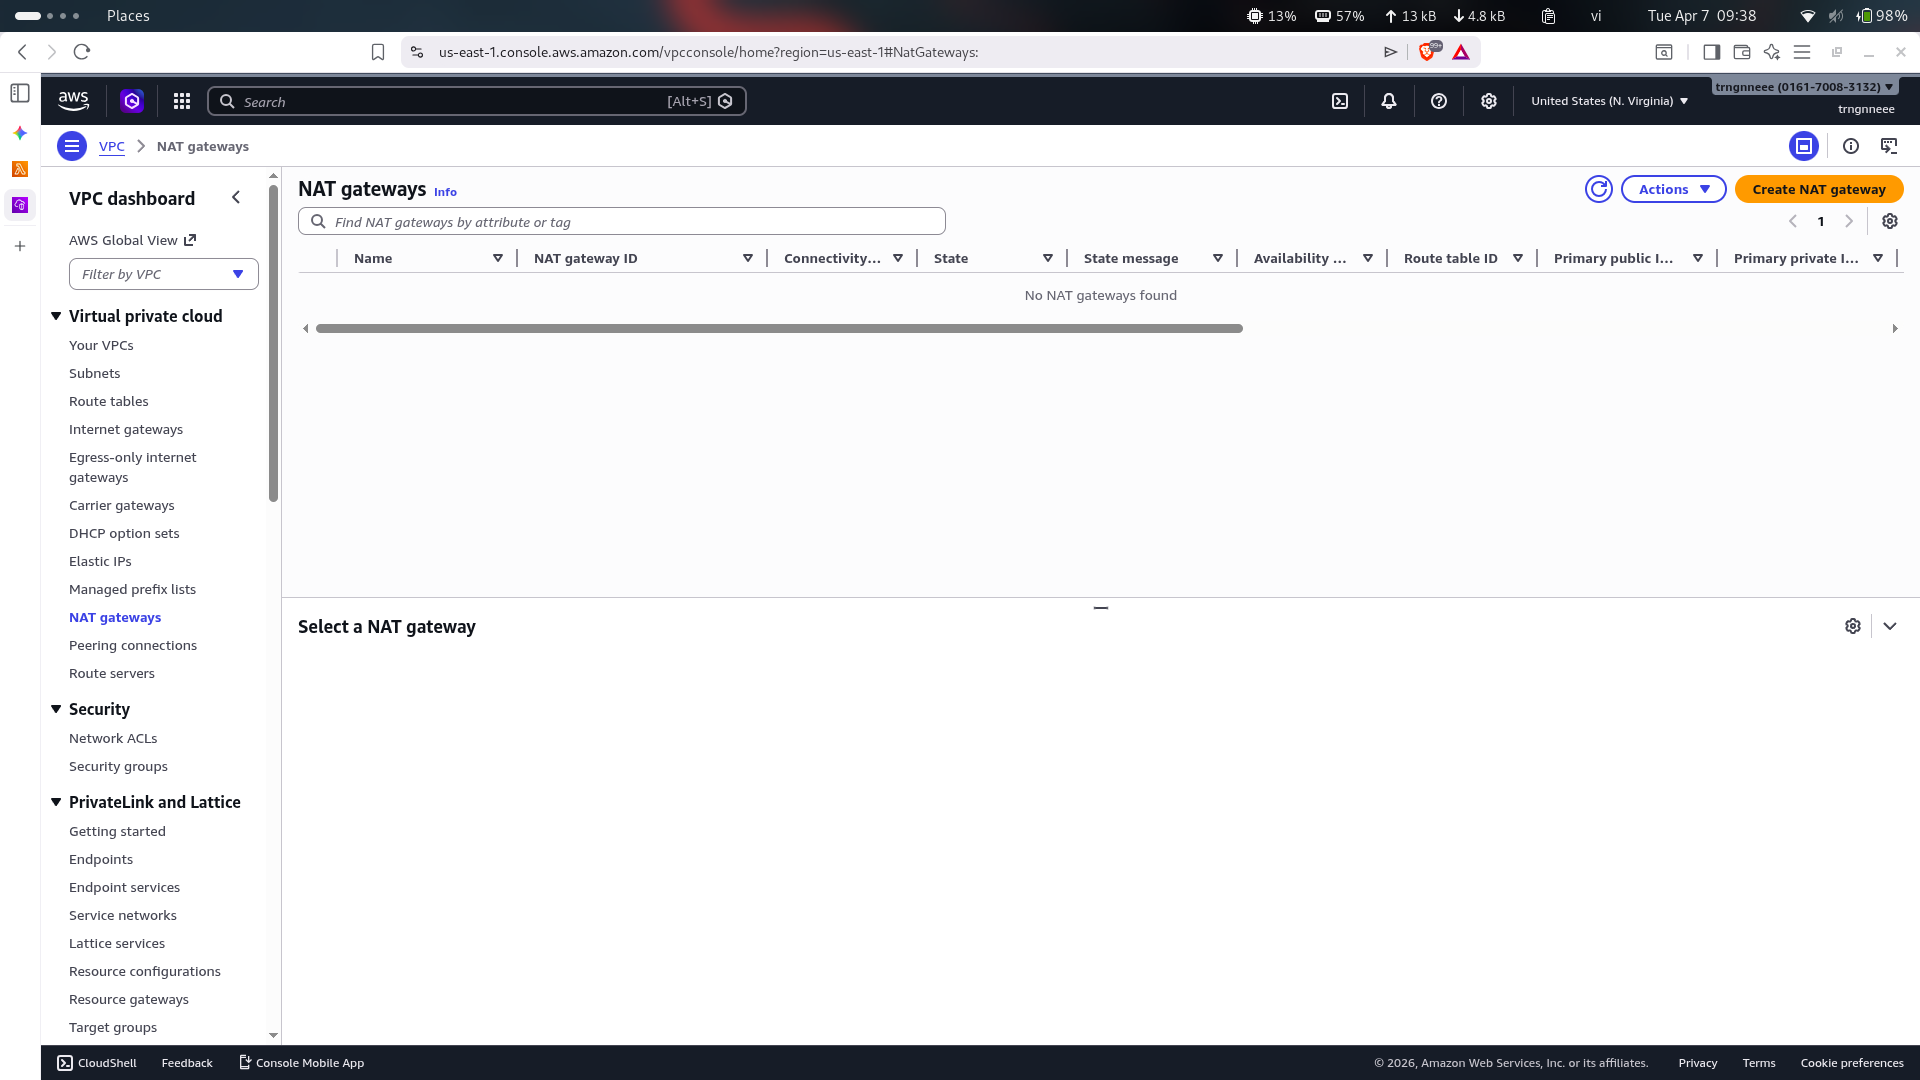
\includegraphics[width=0.8\textwidth]{images/NE4.png}
    \caption{NE-4}
\end{figure}

\subsection{NE-5: Lambda successfully calls DynamoDB}
\begin{figure}[H]
    \centering
    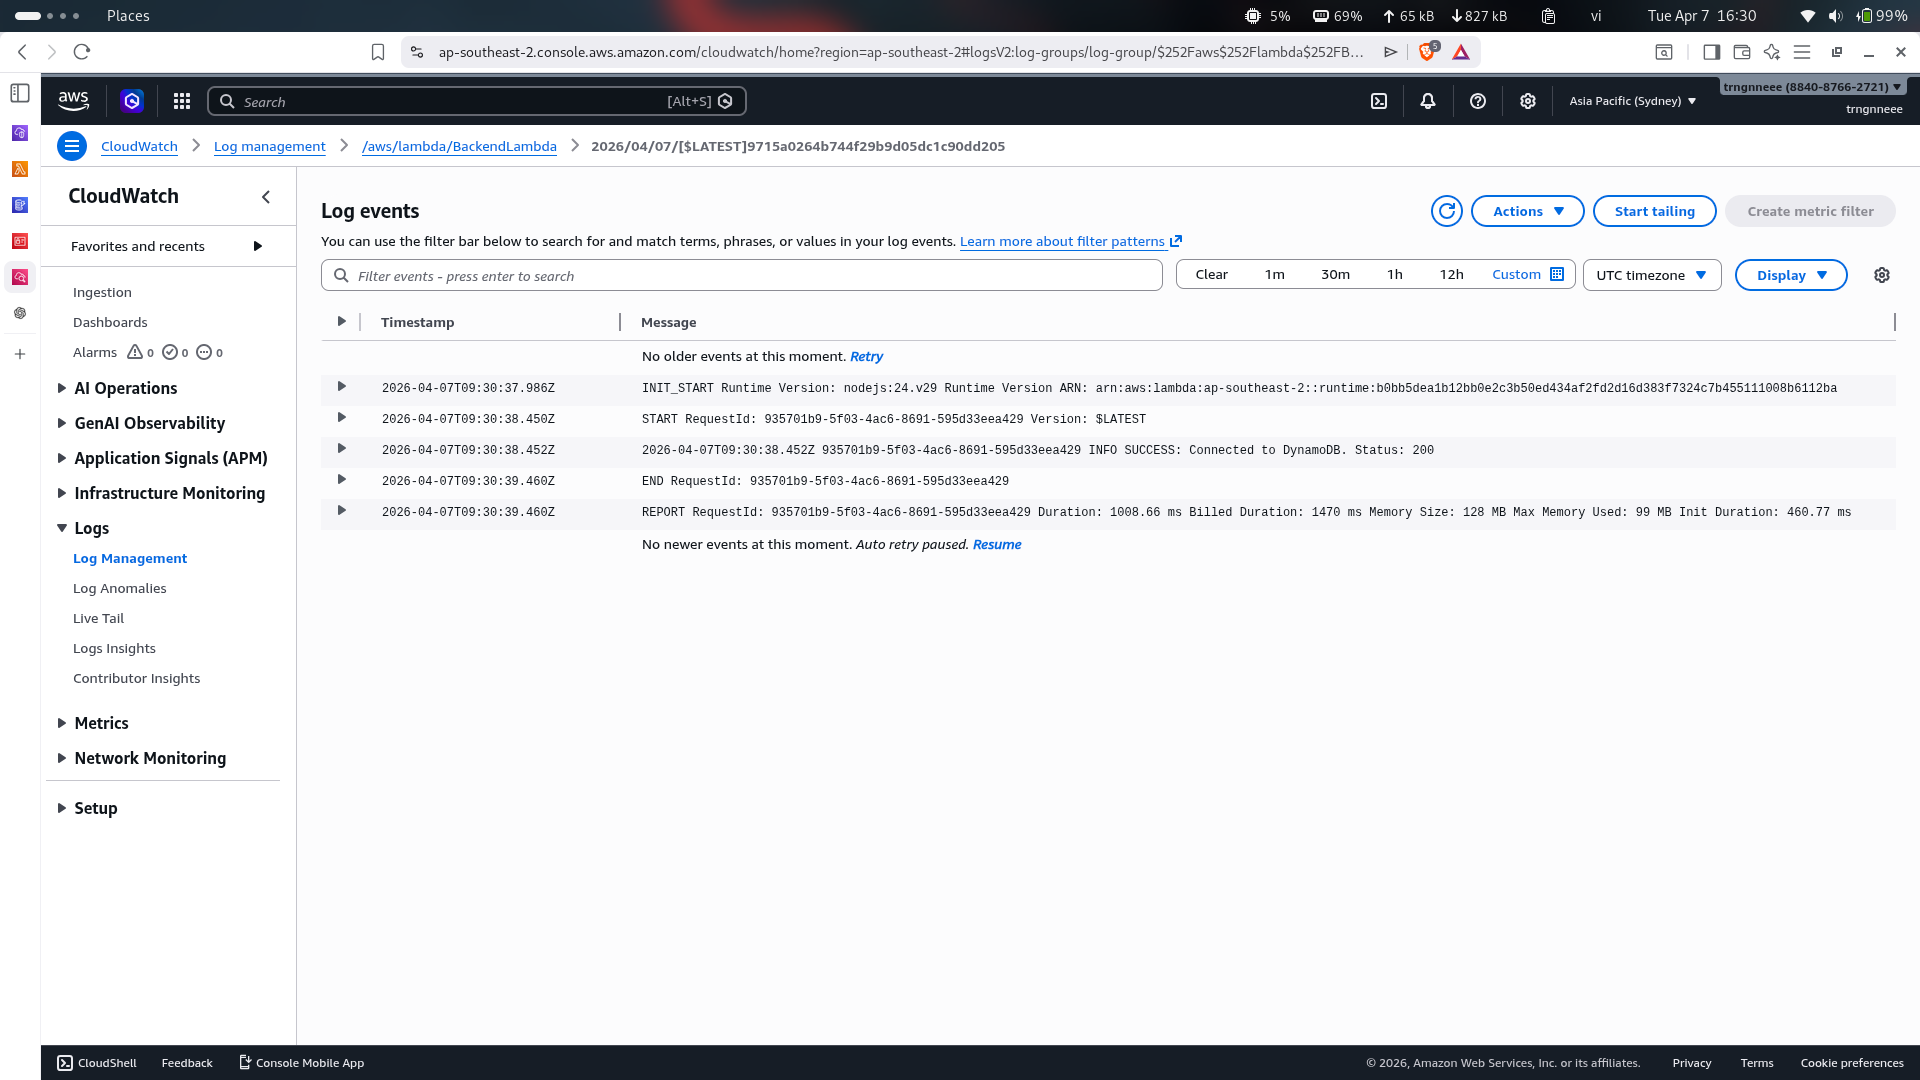
\includegraphics[width=0.8\textwidth]{images/NE5.png}
    \caption{NE-5}
\end{figure}

\section{IAM evidence}


\subsection{IM-1: Two separate IAM Roles}
\begin{figure}[H]
    \centering
    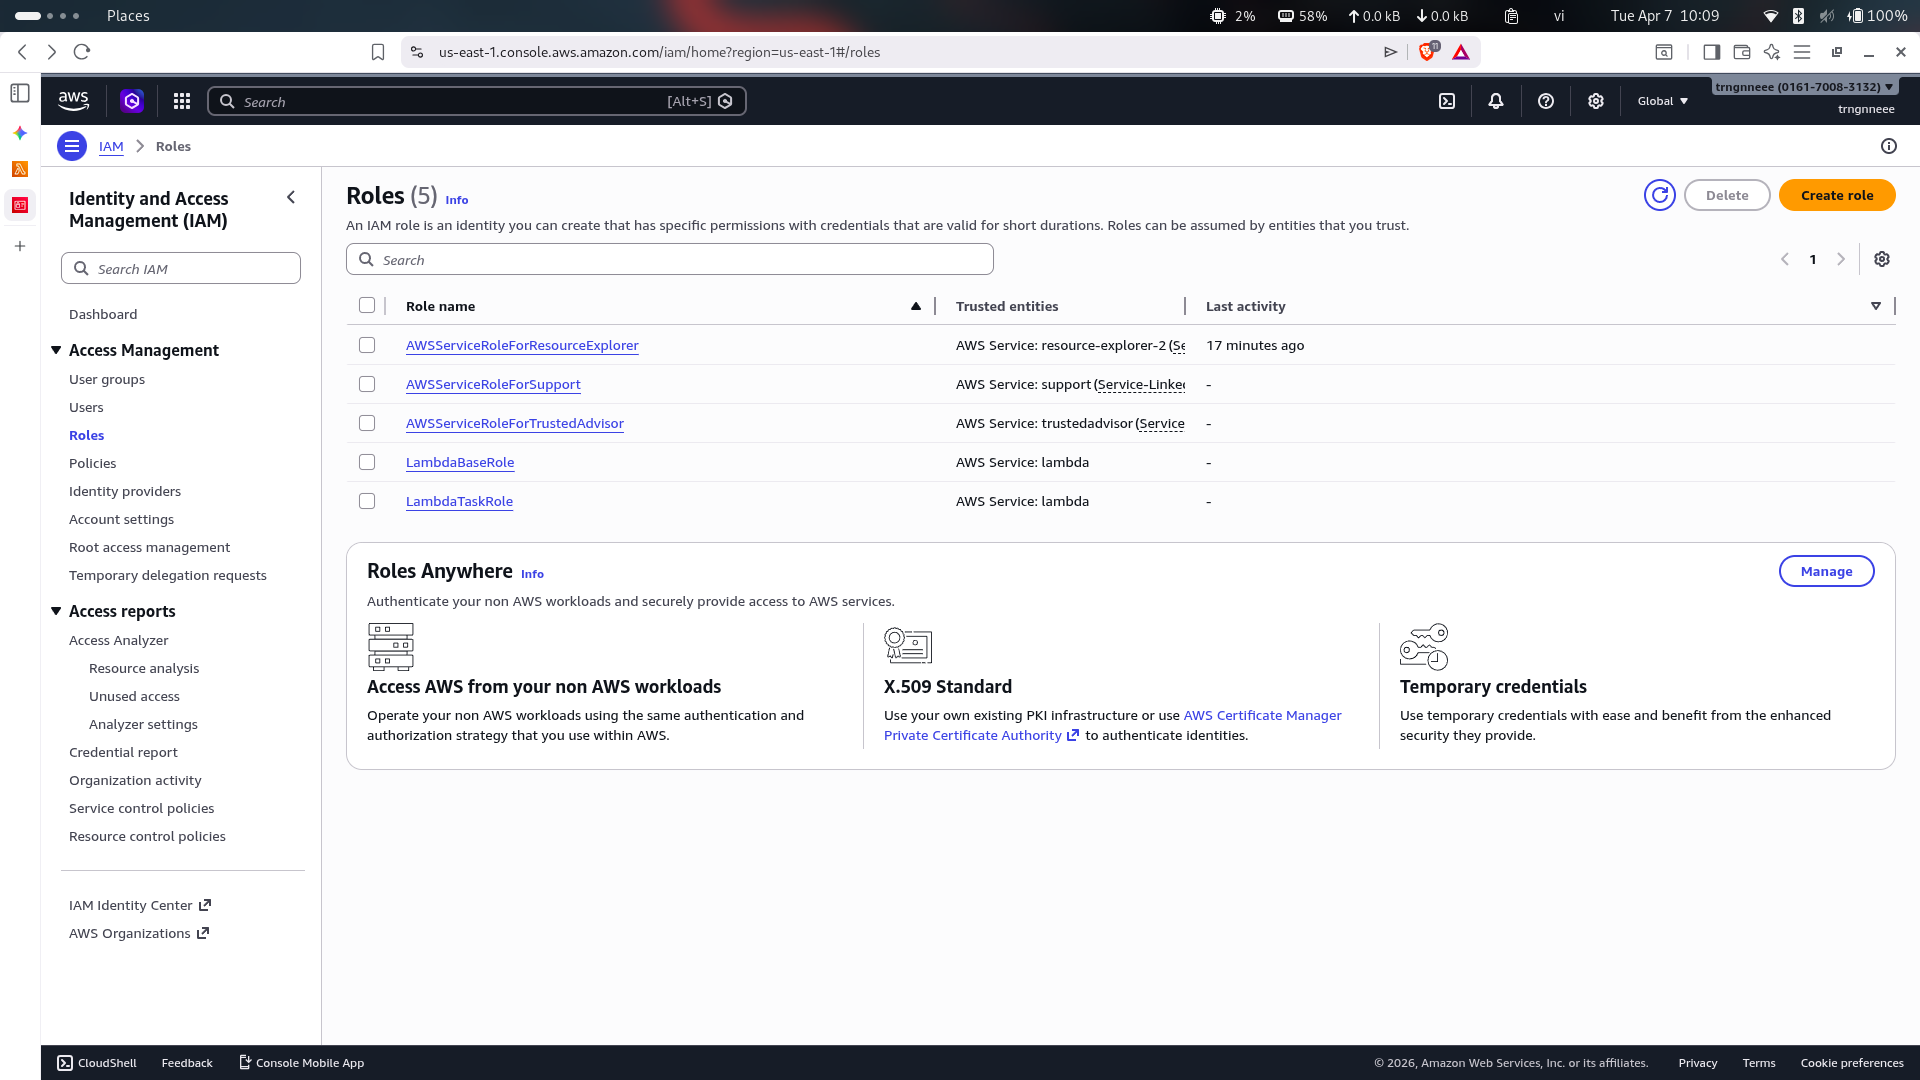
\includegraphics[width=0.8\textwidth]{images/IM1.png}
    \caption{IM-1}
\end{figure}

\subsection{IM-2: Policy specifies exact resource ARN}
\begin{figure}[H]
    \centering
    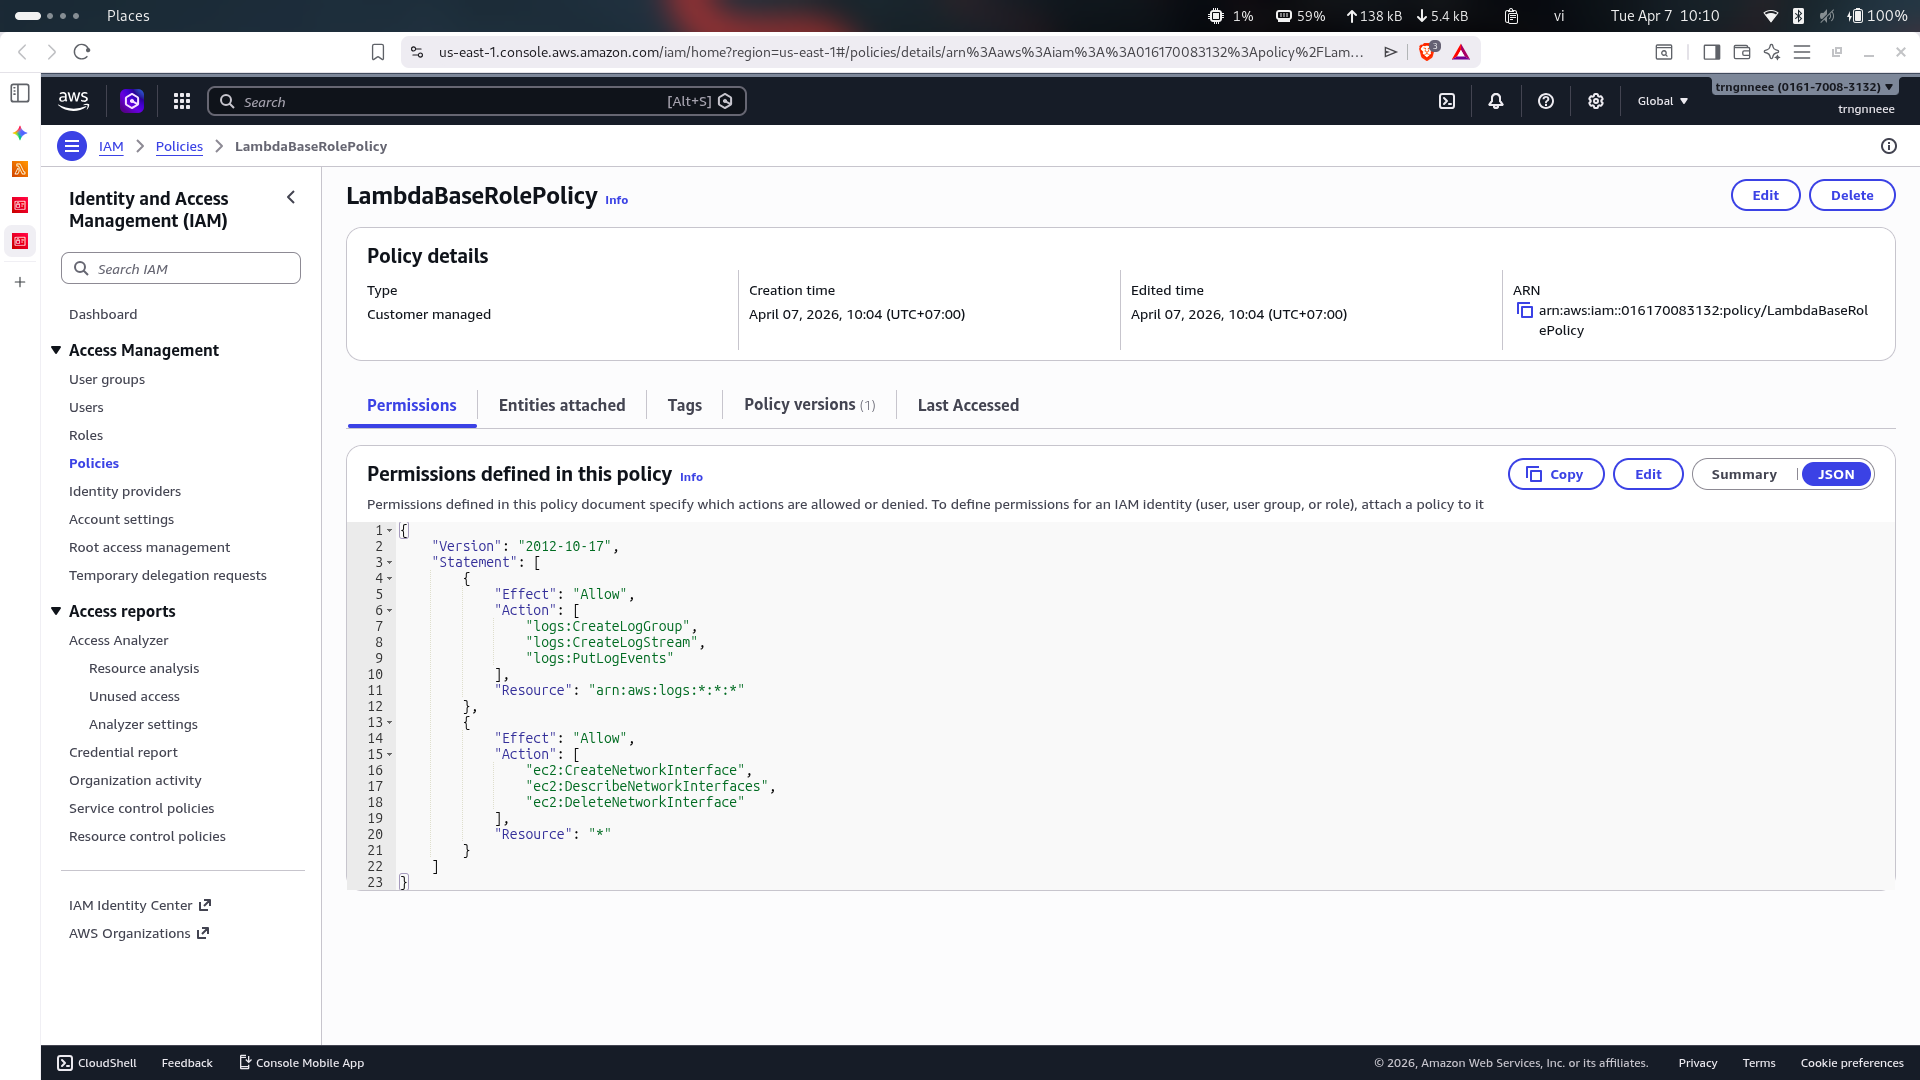
\includegraphics[width=0.8\textwidth]{images/IM2-1.png}
    \caption{Lambda Base Role's Policy}
\end{figure}

\begin{figure}[H]
    \centering
    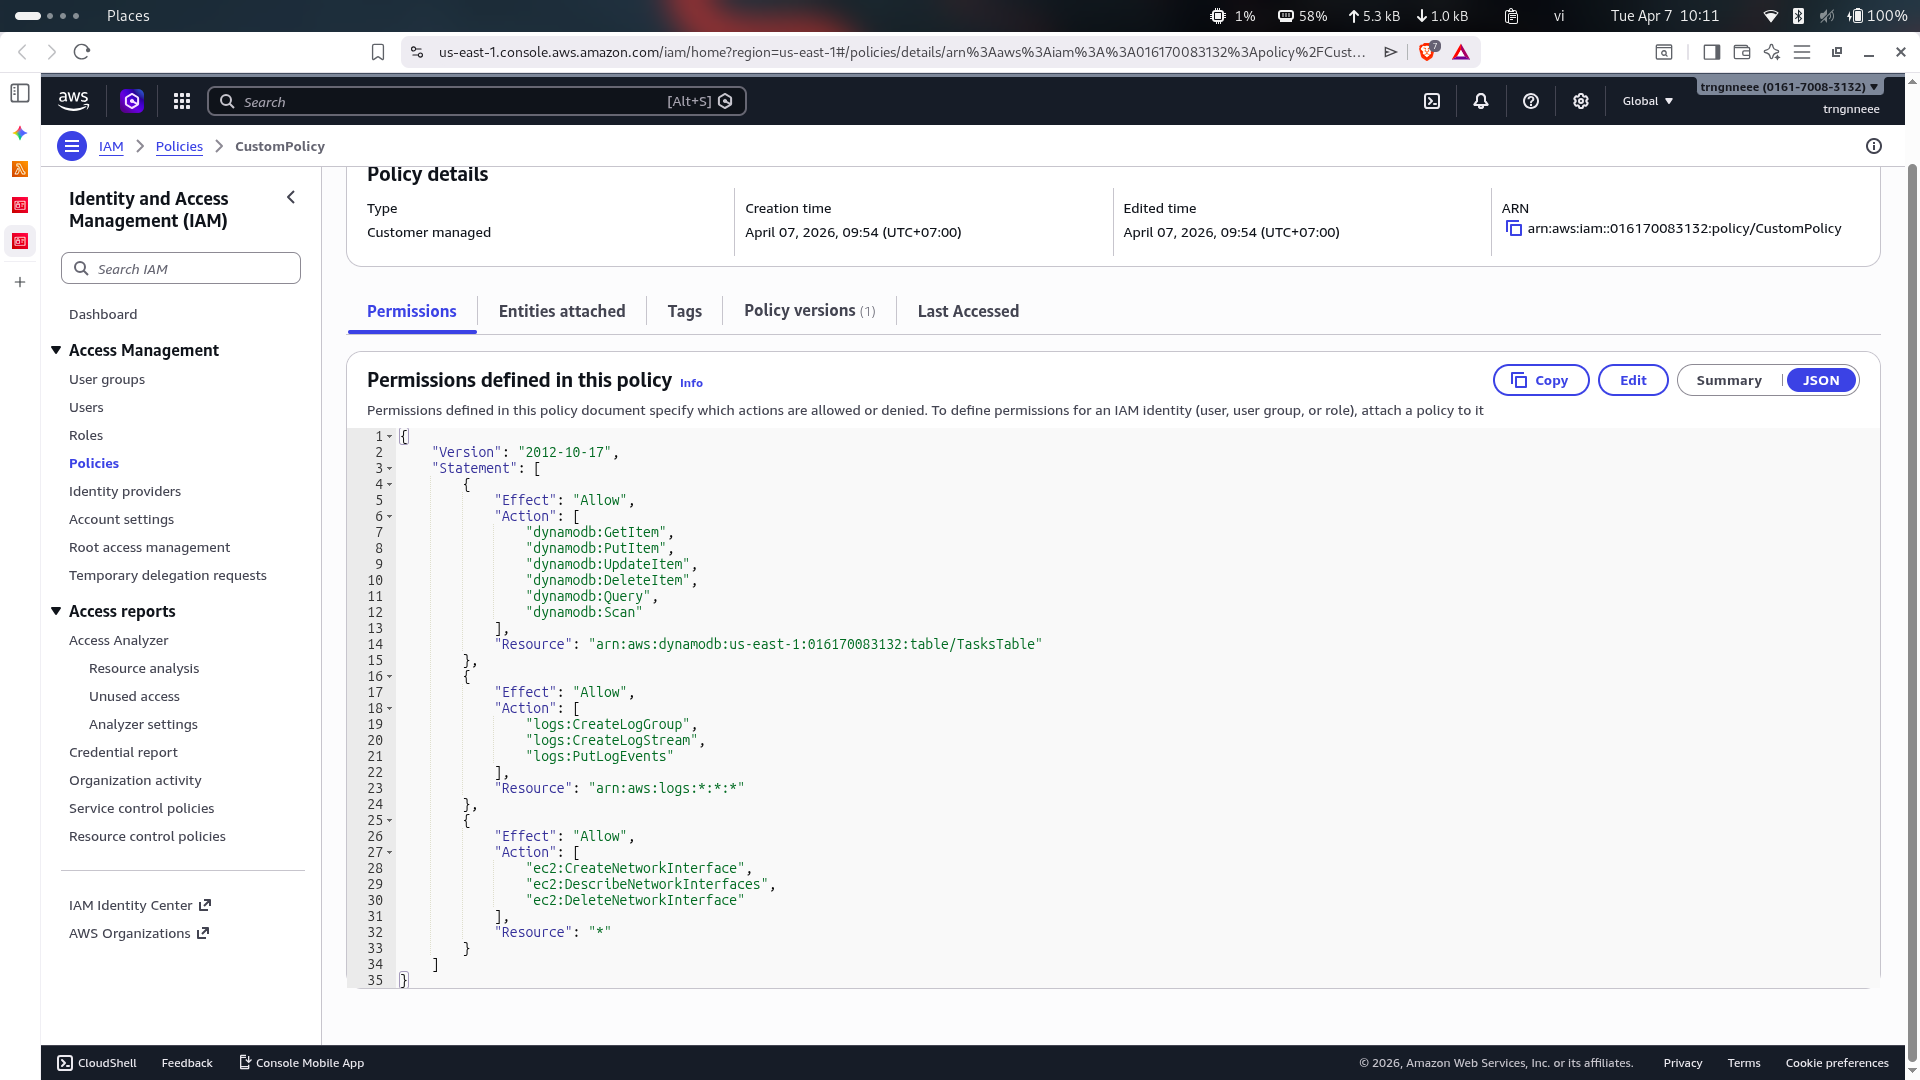
\includegraphics[width=0.8\textwidth]{images/IM2-2.png}
    \caption{Lambda Task Role's Policy}
\end{figure}

\subsection{IM-3: Lambda attached to the correct Role}
\begin{figure}[H]
    \centering
    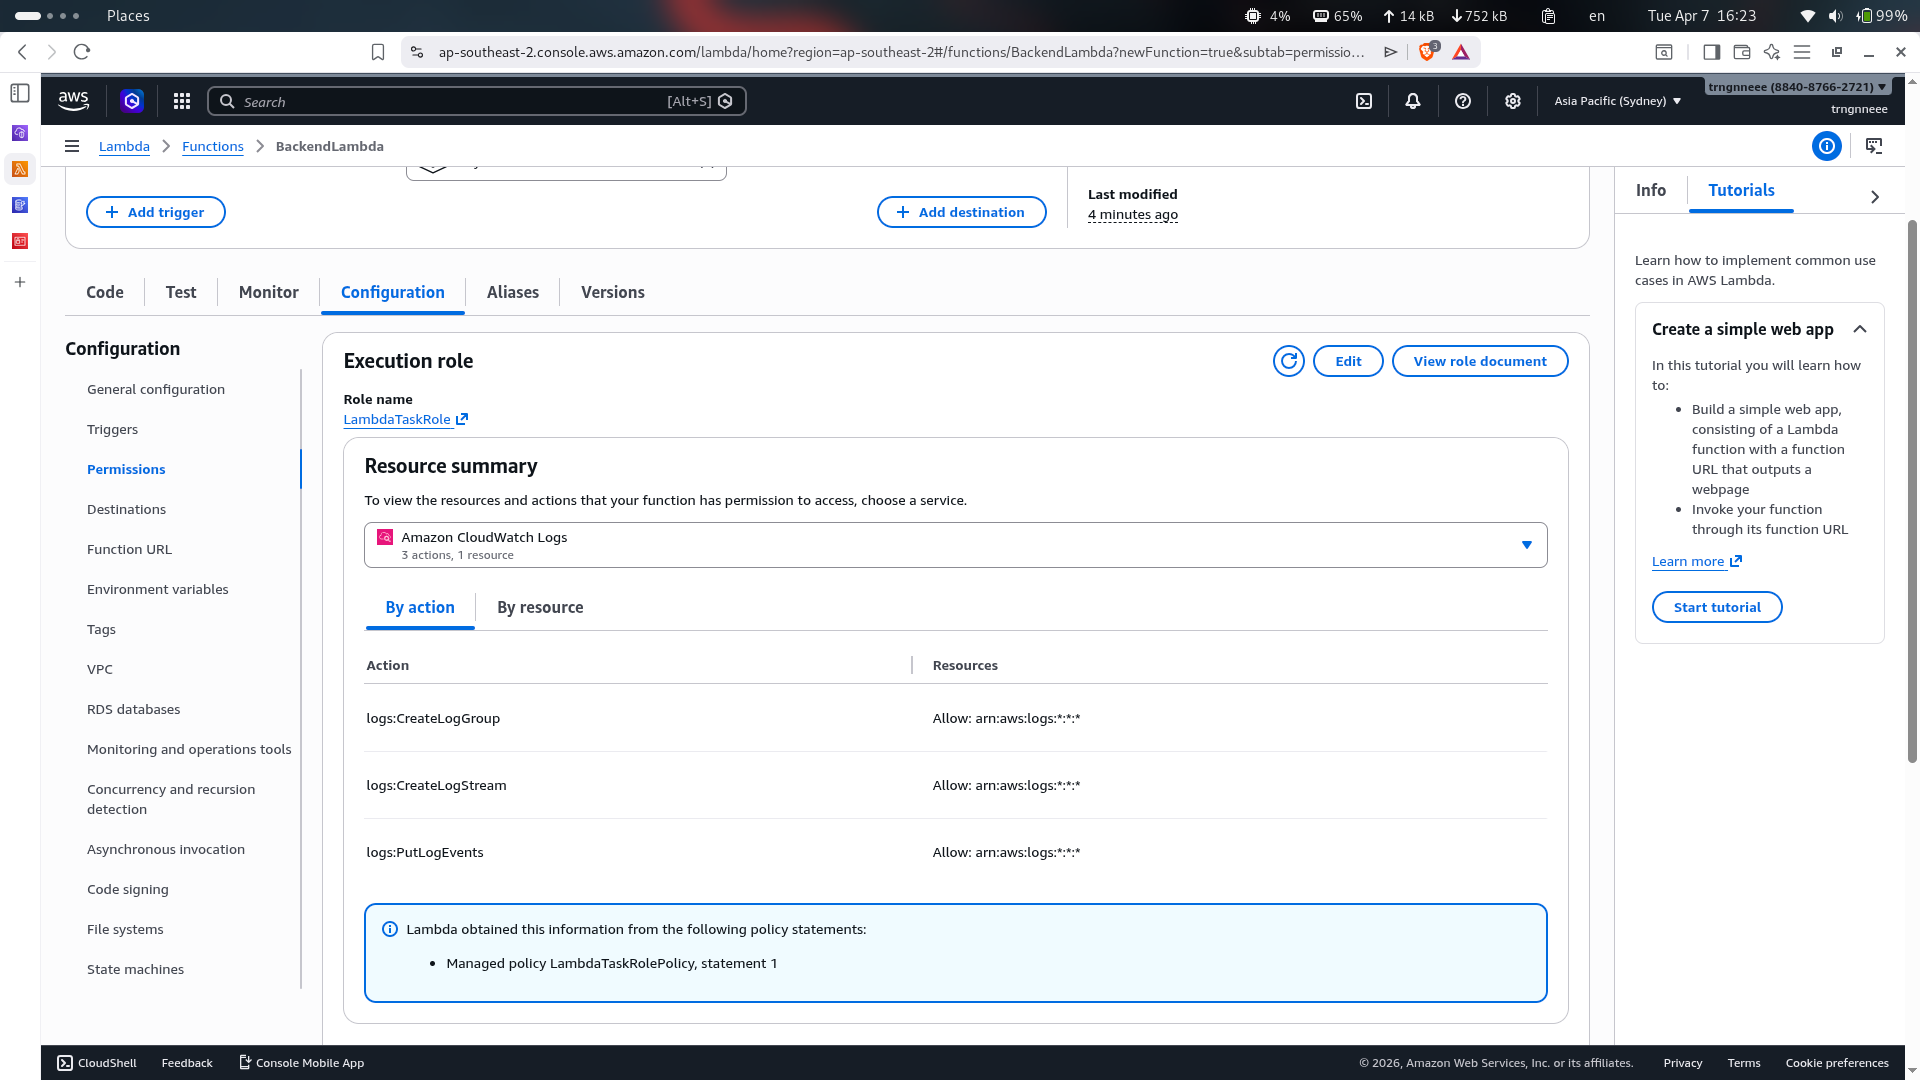
\includegraphics[width=0.8\textwidth]{images/IM3-1.png}
    \caption{Lambda Execution Role by Action}
\end{figure}

\begin{figure}[H]
    \centering
    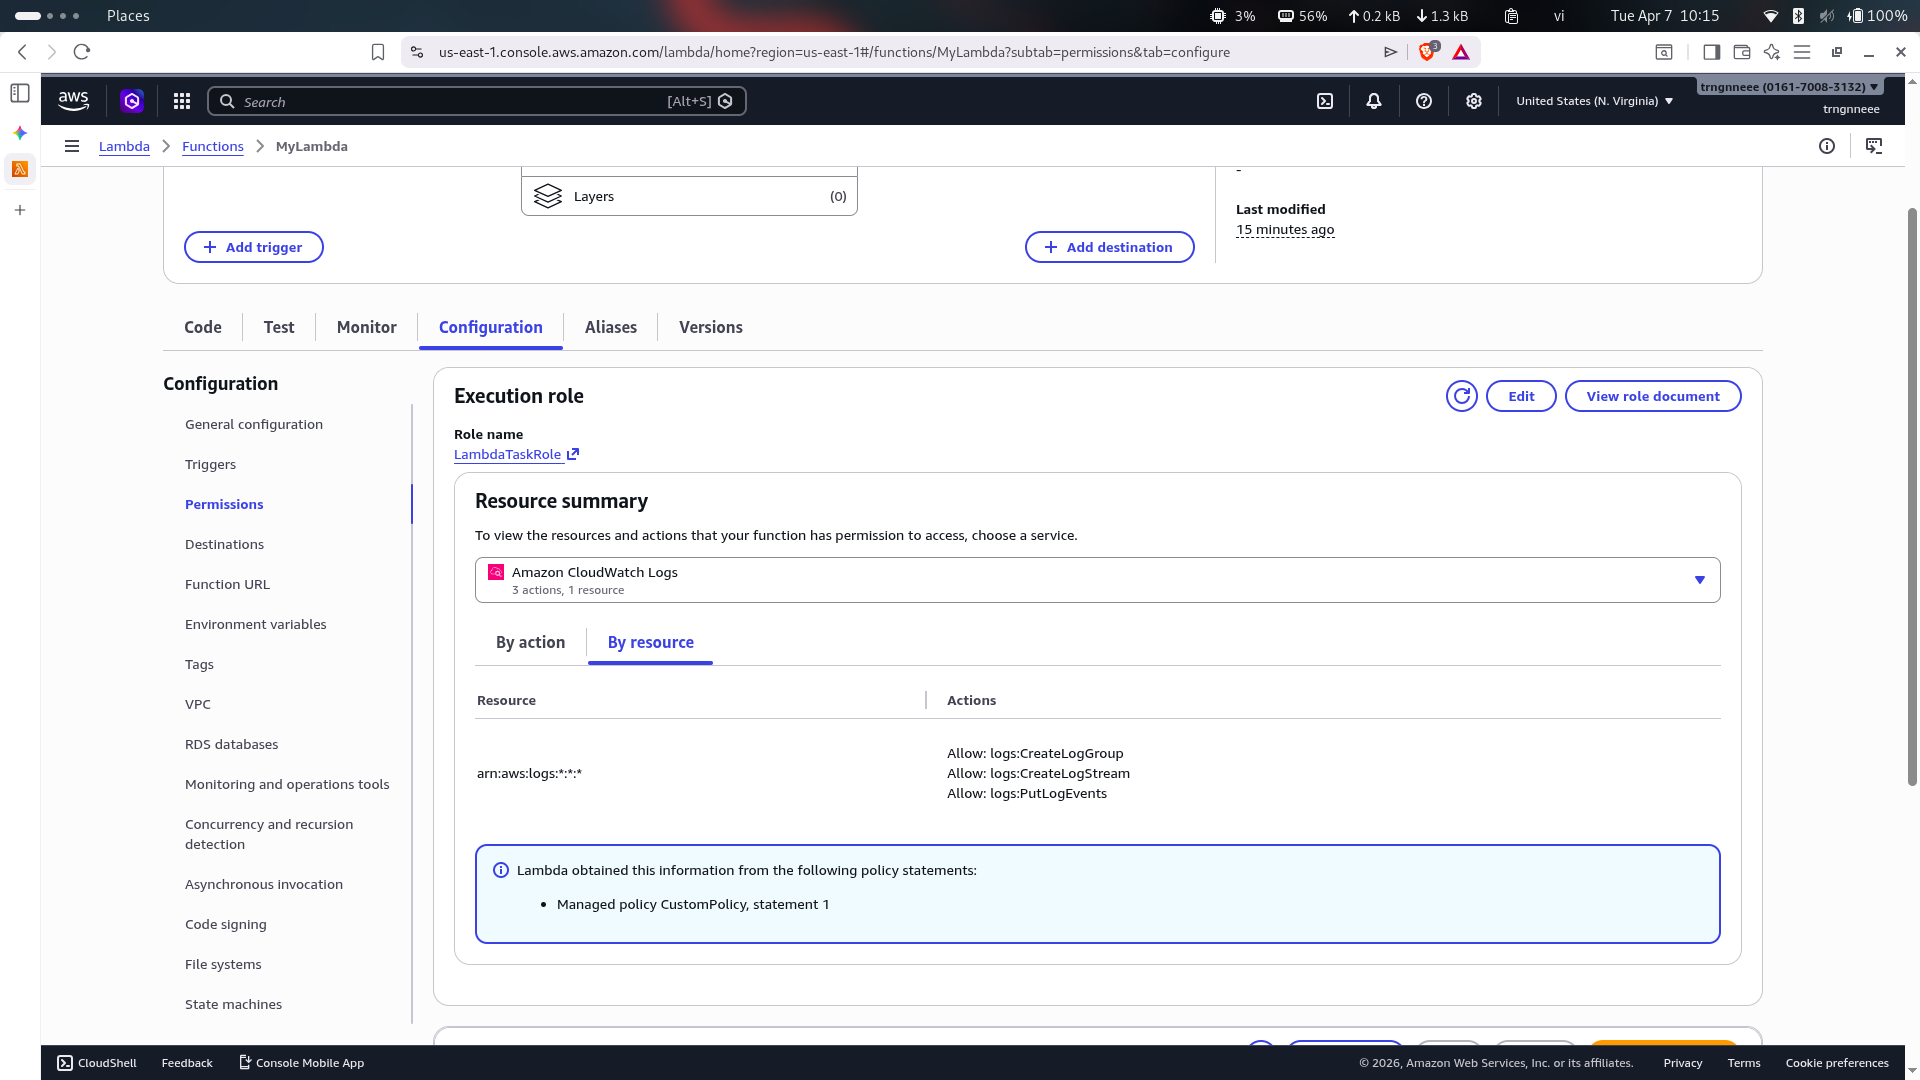
\includegraphics[width=0.8\textwidth]{images/IM3-2.png}
    \caption{Lambda Execution Role by Resources}
\end{figure}

\section{Log evidence}

\subsection{Successful request}
\begin{figure}[H]
    \centering
    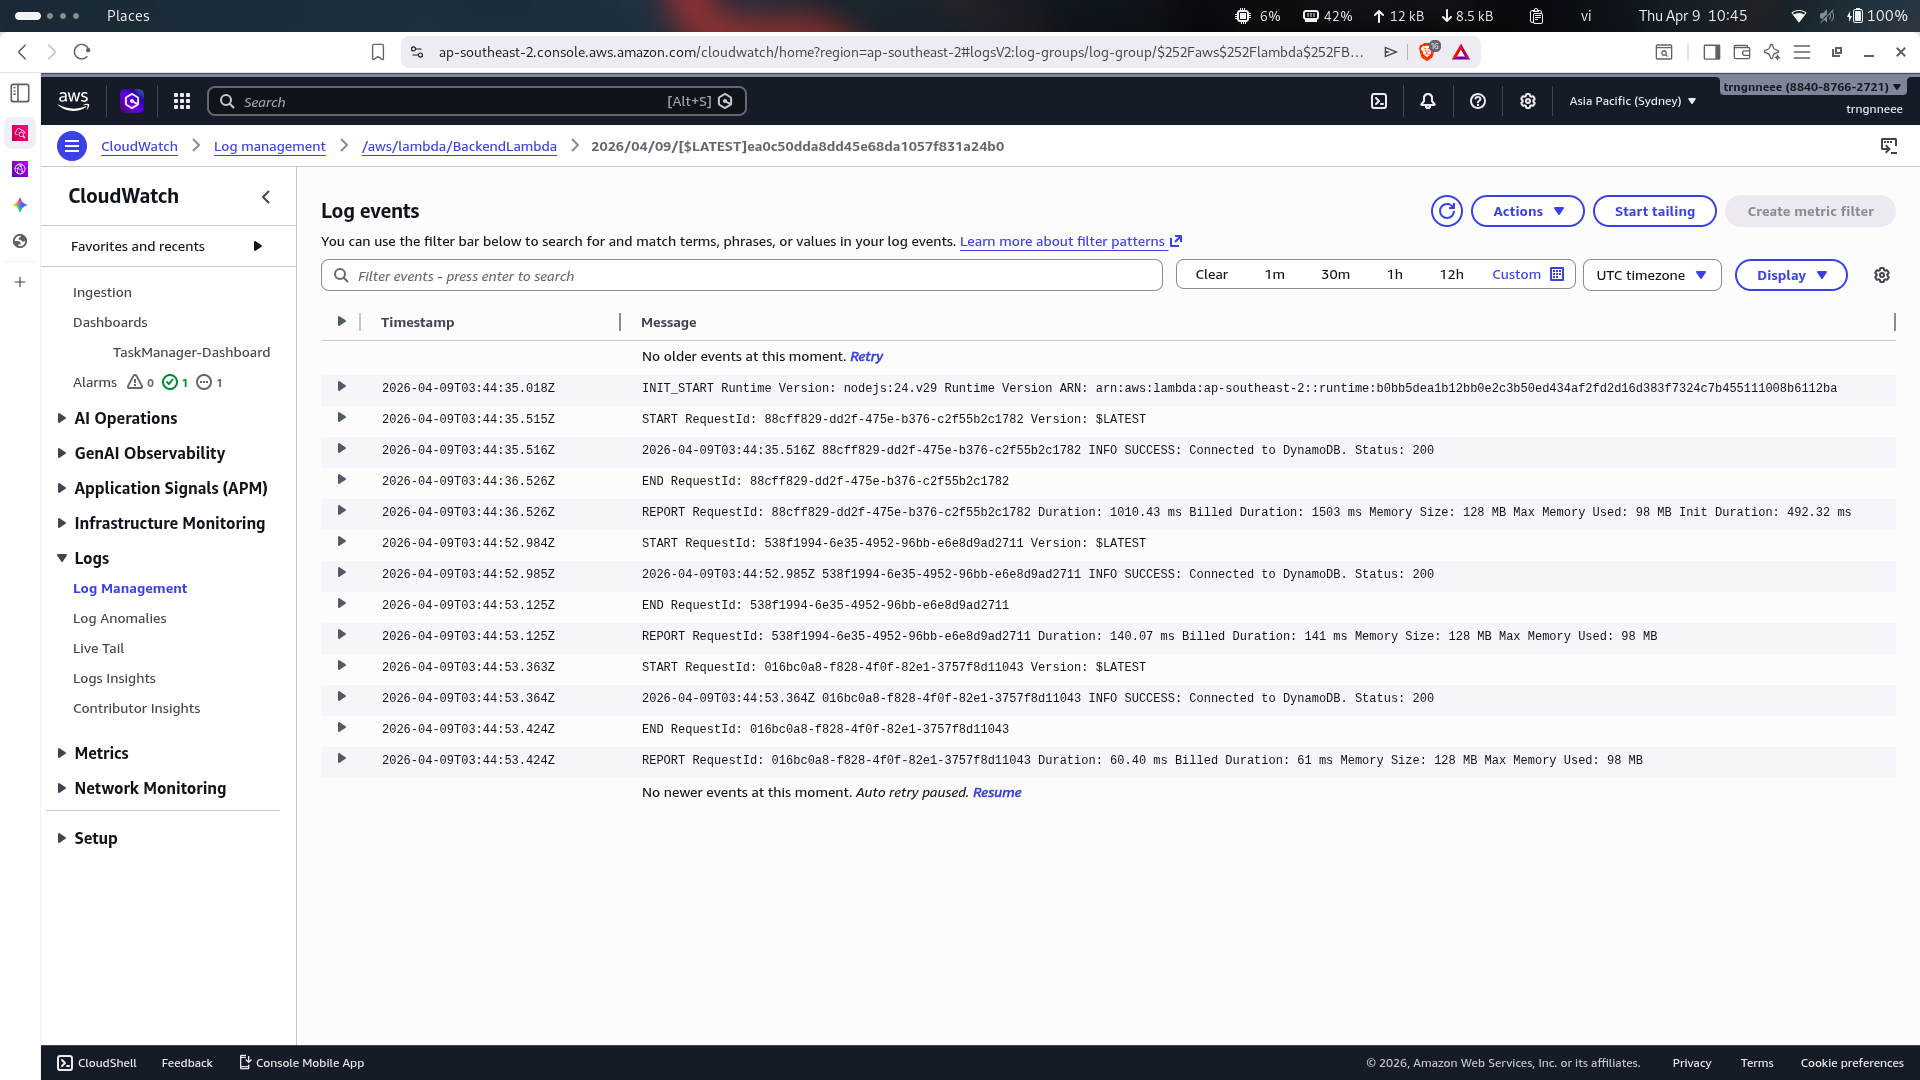
\includegraphics[width=0.8\textwidth]{images/LOG1.png}
    \caption{Log showing the REPORT line with StatusCode 200, Duration, Billed Duration, and Memory Used}
\end{figure}

\subsection{Error request}
\begin{figure}[H]
    \centering
    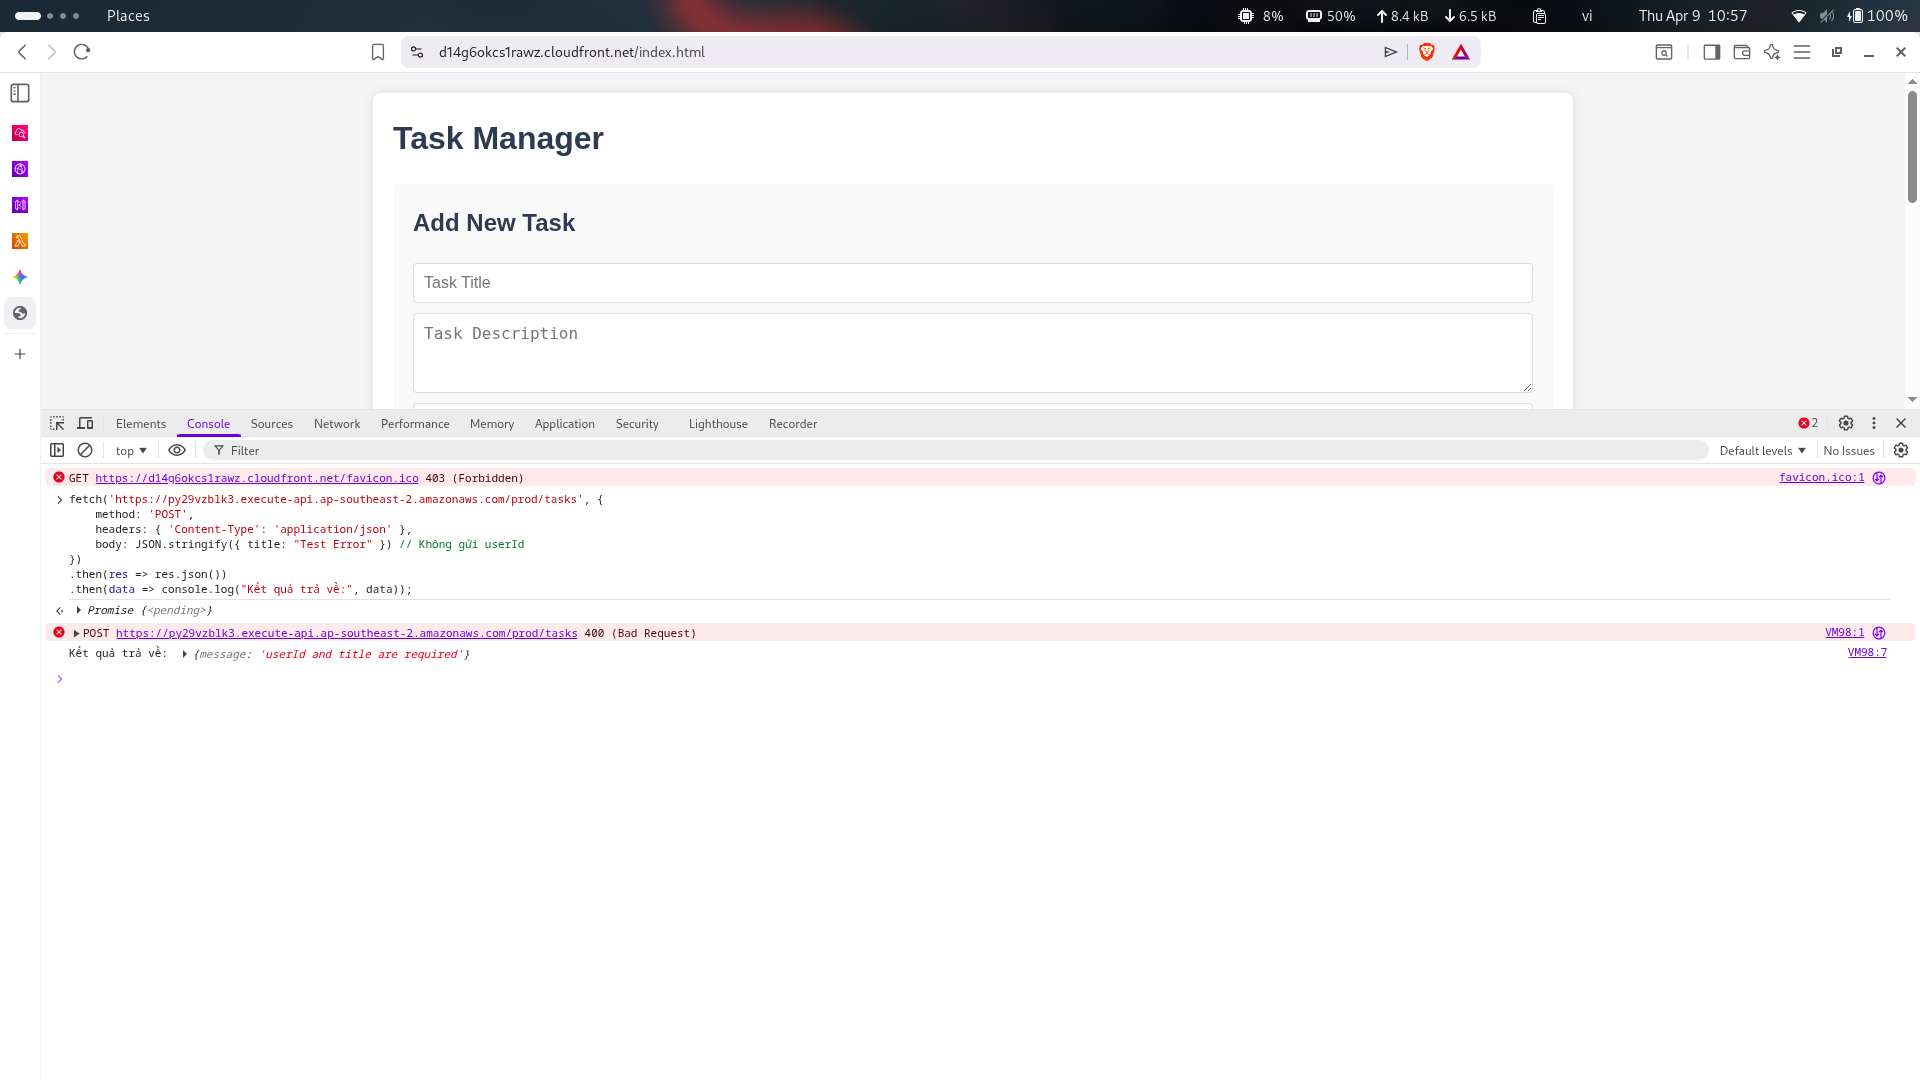
\includegraphics[width=0.8\textwidth]{images/LOG2-1.png}
    \caption{Sending missing input}
\end{figure}
\begin{figure}[H]
    \centering
    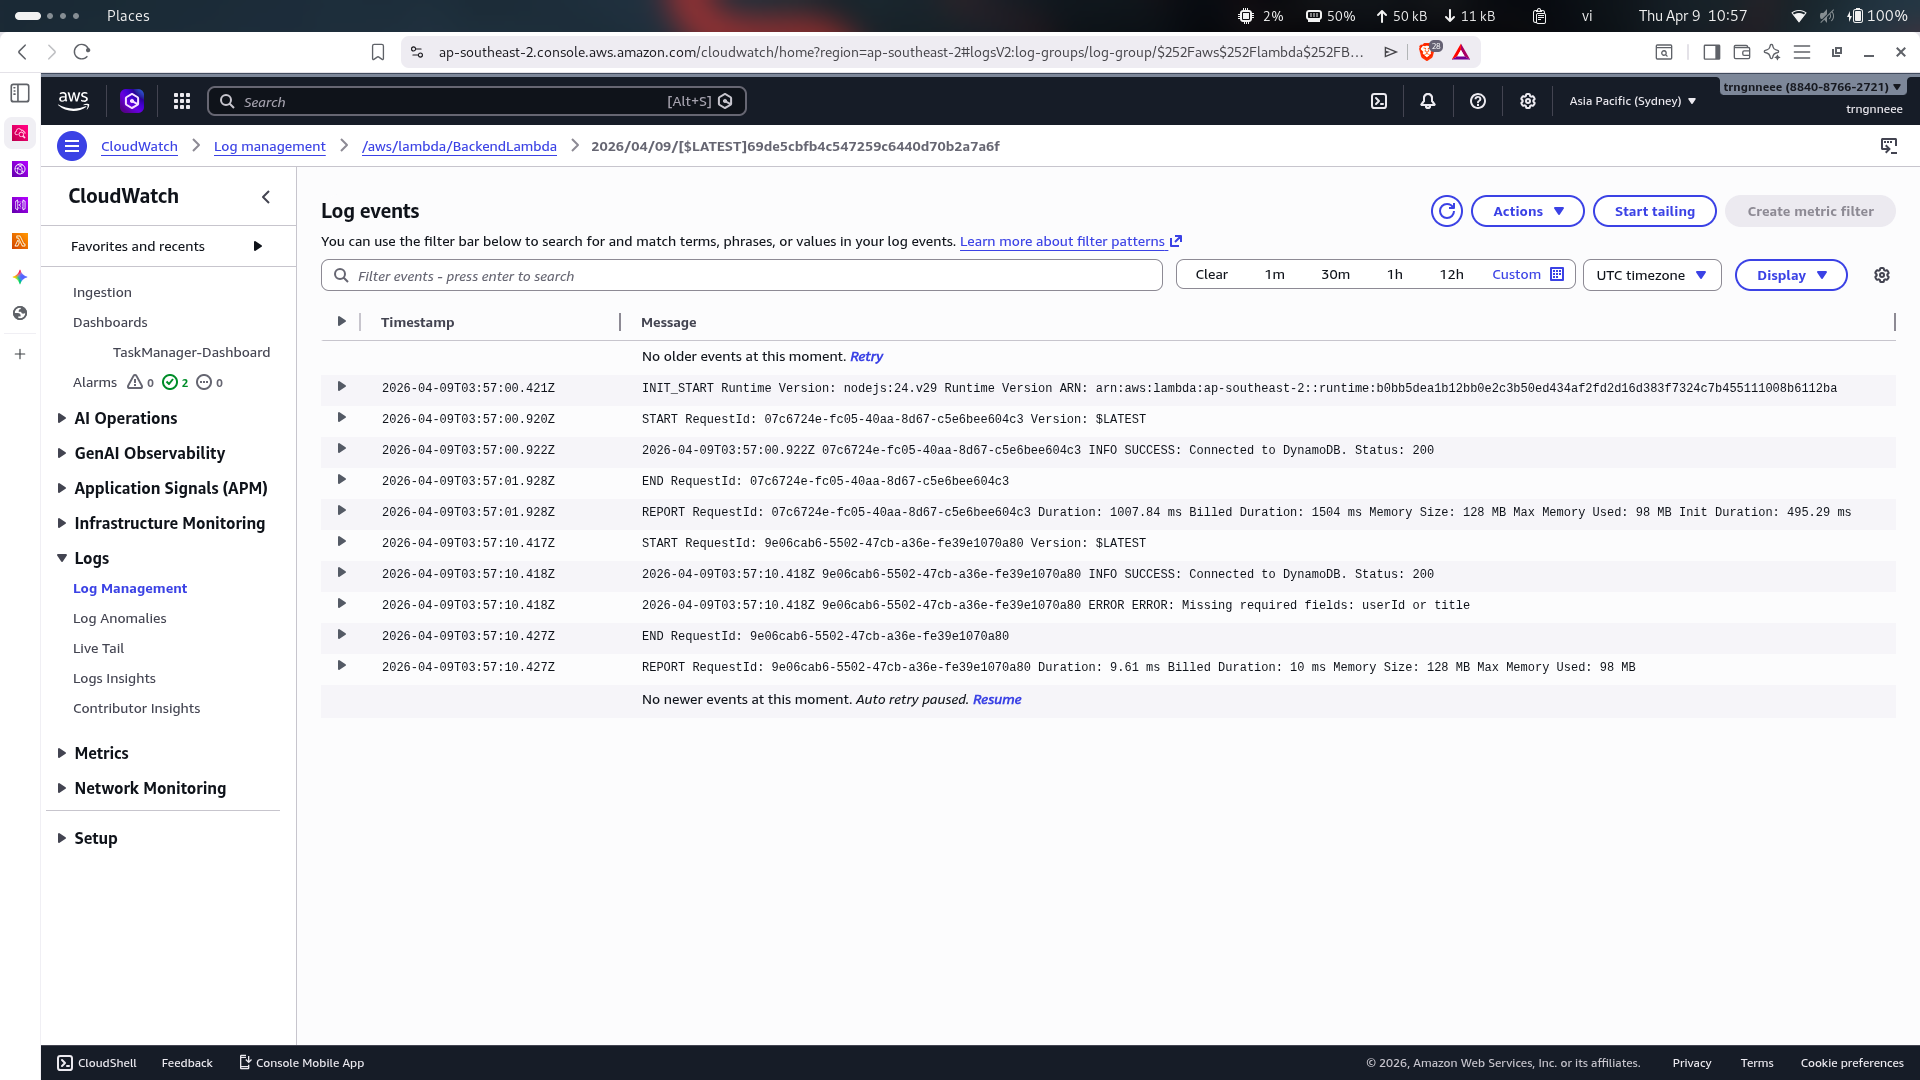
\includegraphics[width=0.8\textwidth]{images/LOG2-2.png}
    \caption{Log showing an ERROR entry or stack trace triggered by sending missing input}
\end{figure}